\documentclass[10pt]{beamer}

\usetheme[sectionpage=none, subsectionpage=progressbar]{metropolis}
\usepackage{appendixnumberbeamer}

\usepackage{ucs}
\usepackage[utf8x]{inputenc}
\usepackage[ngerman]{babel}

\usepackage{booktabs}
\usepackage[scale=2]{ccicons}

\usepackage{pgfplots}
\usepgfplotslibrary{dateplot}

\usepackage{xspace}
\usepackage{dsfont}
\usepackage{graphicx}
\newcommand{\themename}{\textbf{\textsc{metropolis}}\xspace}

\title{Fallstudien II}
%\subtitle{A modern beamer theme}
\date{11. Dezember 2020}
\author{Laura Kampmann, Christian Peters, Alina Stammen}
%\institute{TU Dortmund}
%\titlegraphic{\hfill\includegraphics[height=1.5cm]{logo.pdf}}

\begin{document}

\maketitle

\begin{frame}{Inhalt}
  \setbeamertemplate{section in toc}[sections numbered]
  \tableofcontents
\end{frame}

%\section{Einleitung}

\begin{frame}{Einleitung}
	\begin{itemize}
		\item $\textbf{Motivation}$: Verbesserung mobiler Kommunikation von Endgäten \\
		$\rightarrow$ Vermeiden von z.B. "packet loss" und als Folge auch Retransmission
		\item Wie kann das erreicht werden? \\
		$\rightarrow$ Datenratenprädiktion um optimalen Zeitpunkt zum Senden von Daten zu ermitteln
    \end{itemize}
\end{frame}


\begin{frame}{Datenbeschreibung}
Situation:
	\begin{itemize}
		\item echt Welt Messungen im öffentlichen LTE Netzwerk der 3 deutschen Mobilfunkanbieter o2, T-Mobile und Vodafone
		\item Aufteilung in mehrere Szenarien: "campus", "urban", "suburban" und "highway"
		\item pro Mobilfunkanbieter und Szenario wurden 10 Testfahrten durchgeführt
	\end{itemize}
\end{frame}


\begin{frame}{Datenbeschreibung}
	\begin{itemize}
		\item "context": passive Messungen 1s\\
		$\rightarrow$ $\textbf{RSRP}$ \\
		$\rightarrow$ $\textbf{RSRQ}$ \\
		$\rightarrow$ $\textbf{CQI}$ \\
		$\rightarrow$ $\textbf{TA}$ \\
		$\rightarrow$ $\textbf{velocity}$ \\
		$\rightarrow$ $\textbf{Cell ID}$  \\
		$\rightarrow$ $\textbf{payload size}$ \\
		\item "ul" / "dl": aktive Messungen 10s \\
		$\rightarrow$ $\textbf{throughput}$ - Datenrate \\
		\item "cells":
		$\rightarrow$ RSRP / RSRQ der Nachbarzellen
	\end{itemize}
\end{frame}





%\section{Task I: Data Rate Prediction}
\begin{frame}{Task I: Data Rate Prediction}
    \begin{itemize}
        \item Ziel: Evaluation von neuen \textit{anticipatory vehicular communication systems} durch m\"oglichst
            realit\"atsnahe Simulationen \cite{IEEE}
            \begin{itemize}
                \item[$\Rightarrow$] Ansatz: \textit{Data-Driven Network Simulation}
            \end{itemize}
        \item Durch Machine Learning Modelle sollen m\"oglichst realistische Vorhersagen der Datenraten generiert werden
        \item Hoffnung: Bessere Aussagekraft der Simulationen durch Einsatz echten Datenmaterials
    \end{itemize}
\end{frame}


\section{Task I - Vorhersage der Datenrate}

\subsection{Extreme Gradient Boosting}

\begin{frame}{Extreme Gradient Boosting}
    Intro
\end{frame}

\begin{frame}{Features}
    Features
\end{frame}

\begin{frame}{Tuning}
    Tuning
\end{frame}

\begin{frame}{Validierung}
	\begin{figure}[h]
		\centering
		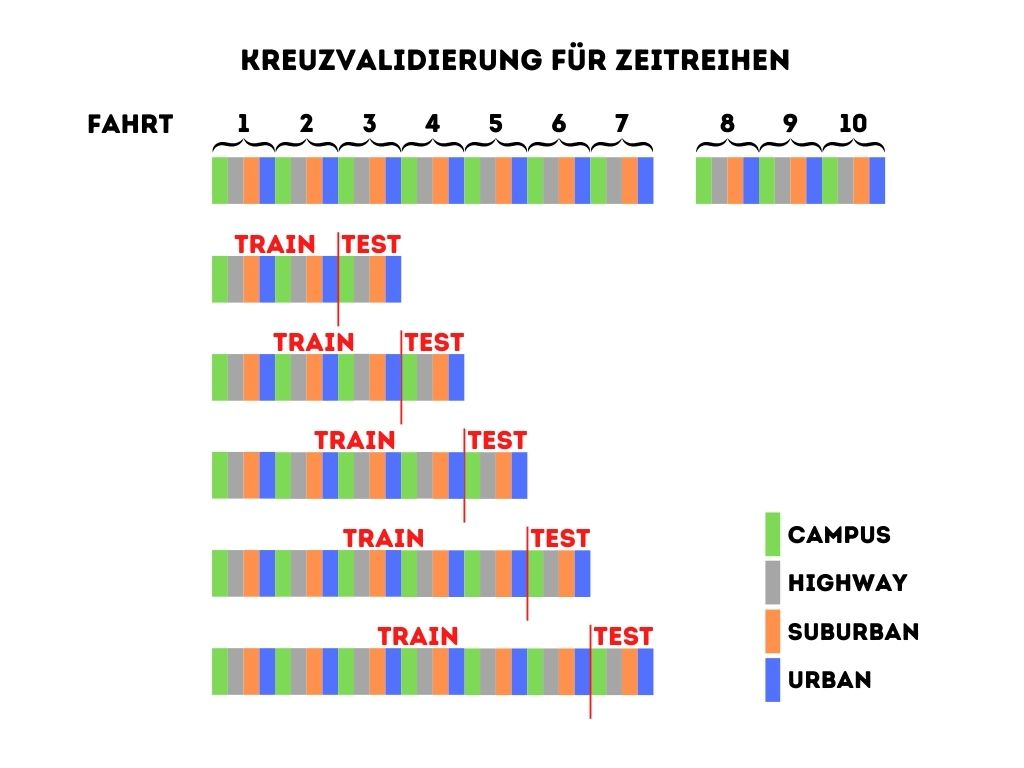
\includegraphics[scale=0.33]{kreuzvalidierung}
		\caption{Einteilungen in Trainings- und Testdatensätze bei der Kreuzvalidierung für Zeitreihen.}
		\label{kreuzvalidierung}
	\end{figure}
\end{frame}

\begin{frame}{Out-of-Sample Vorhersagen}
    \begin{figure}[h]
        \centering
        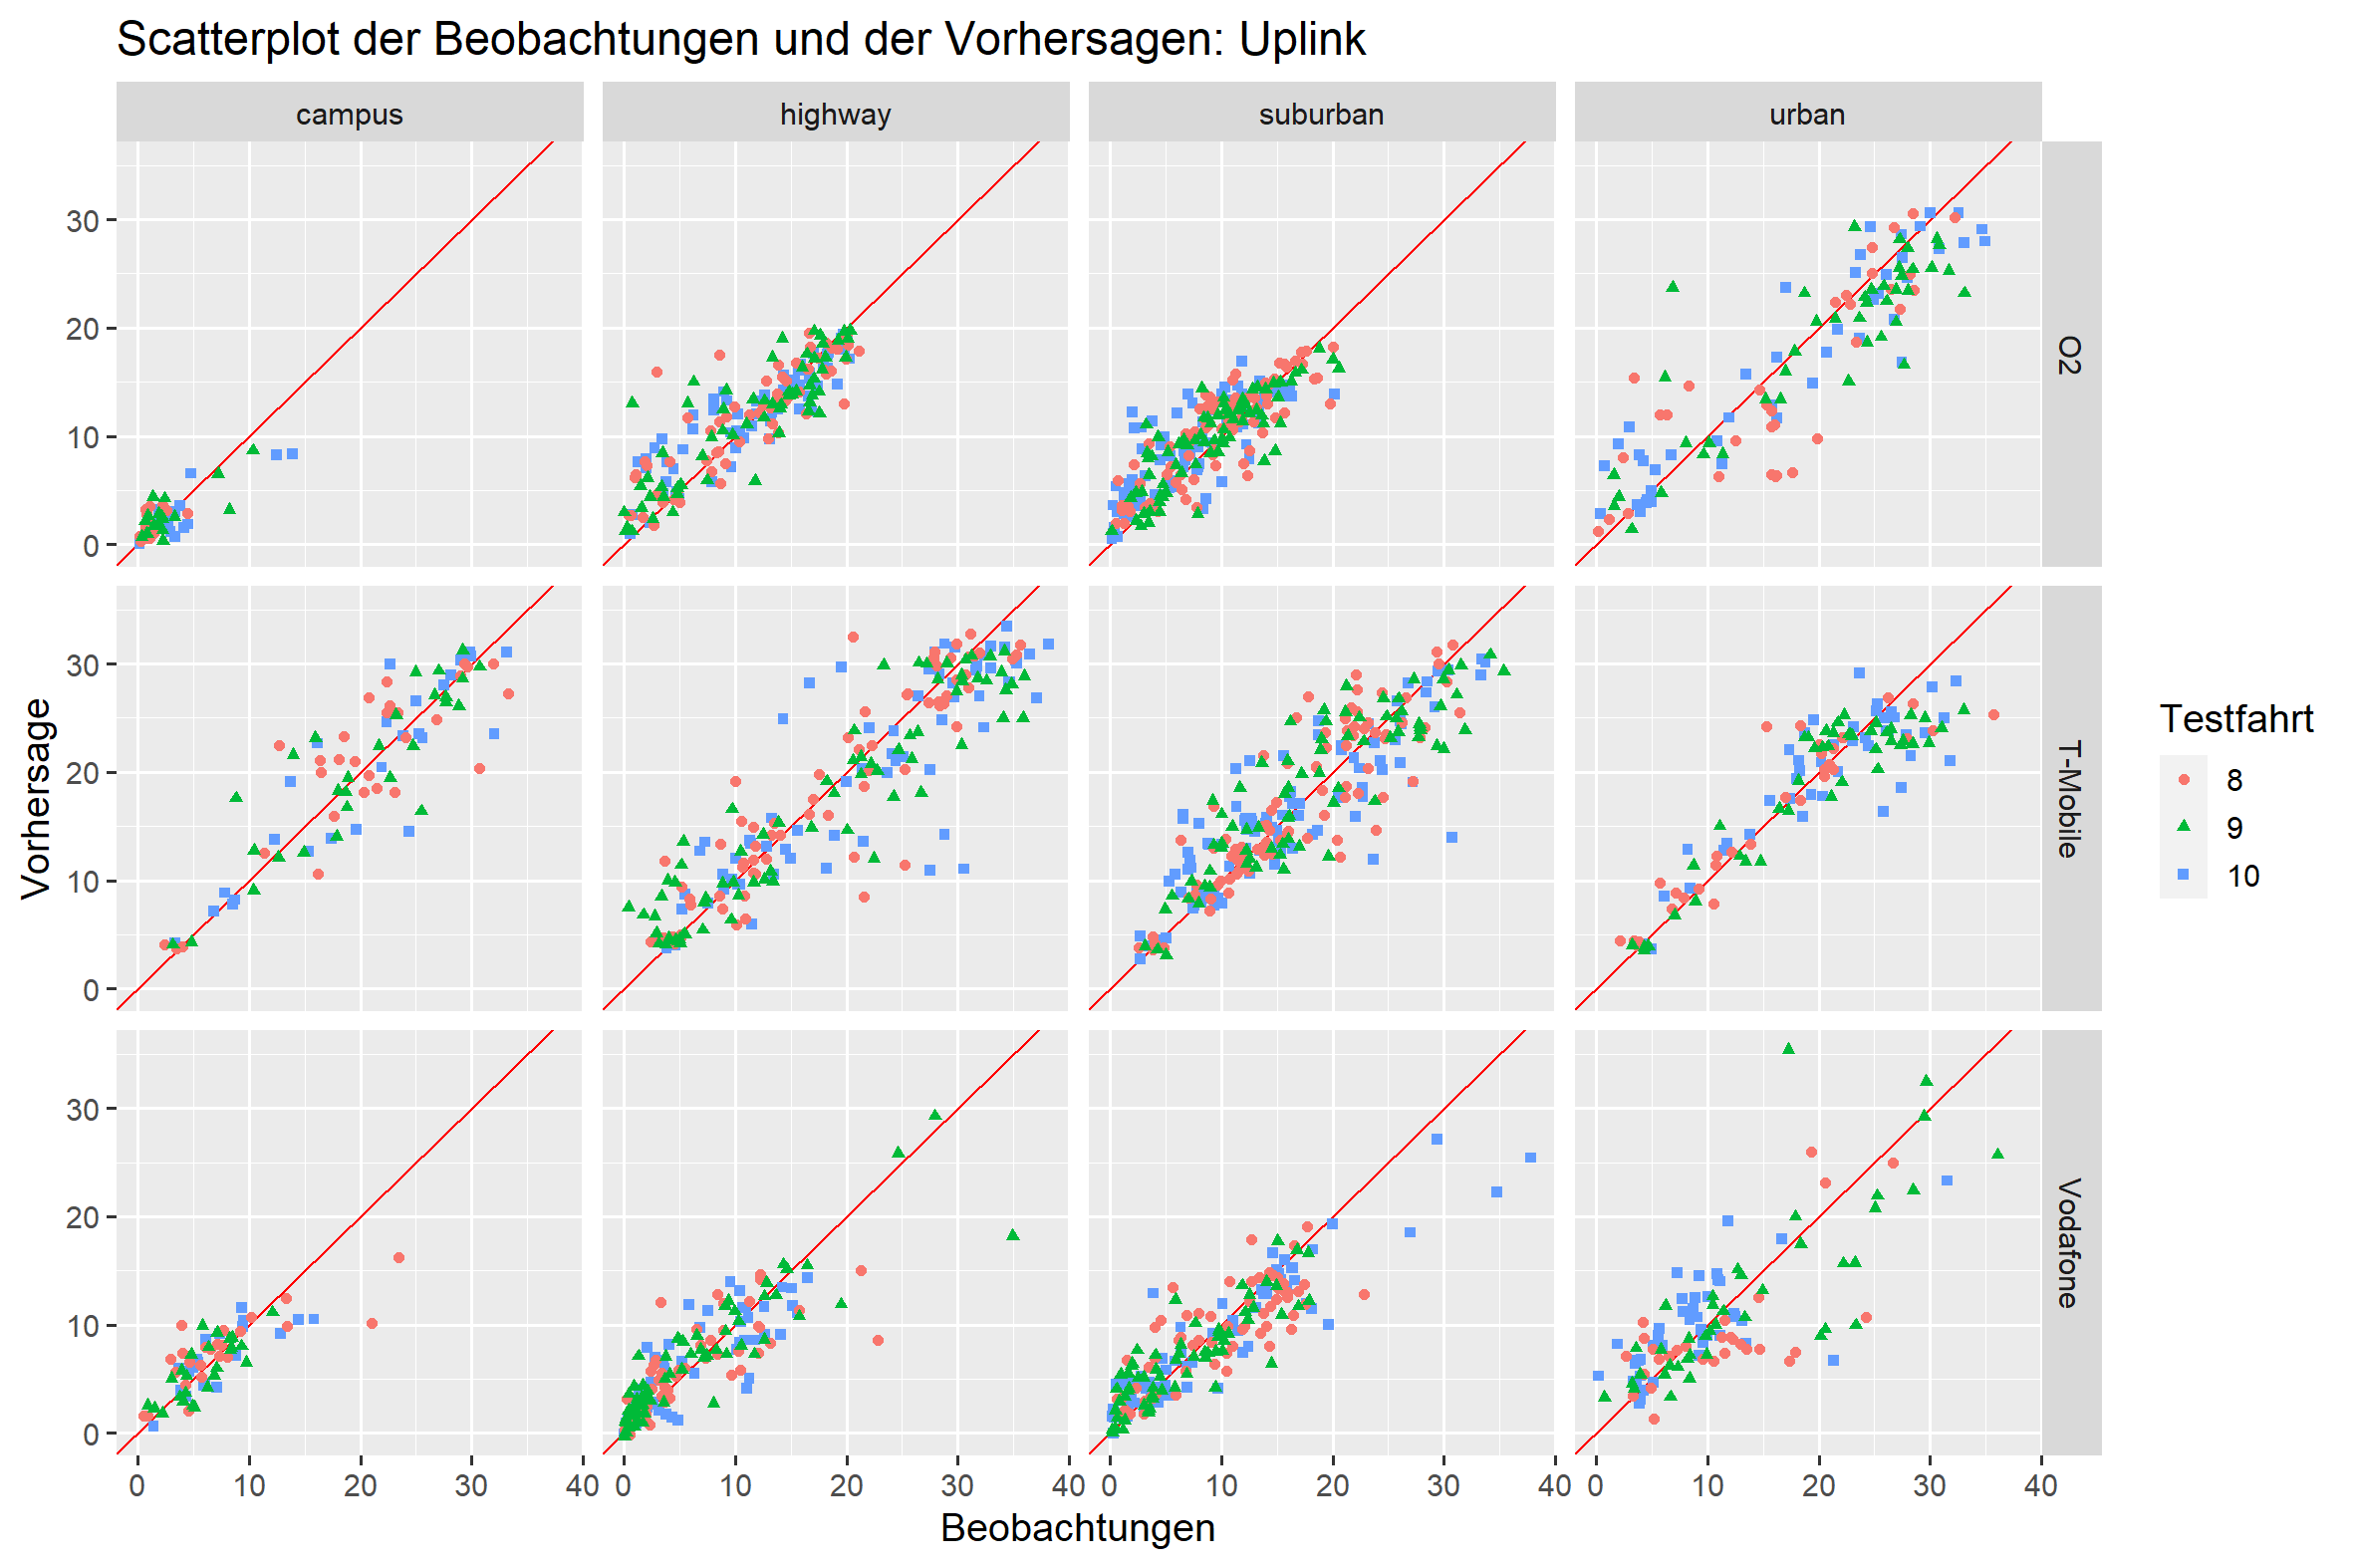
\includegraphics[scale=0.33]{plots/xgboost/uplink/scatter_colored_axes_fixed}
        \caption{XGBoost Out-of-Sample Vorhersagen der Upload-Rate}
        \label{xgboost_scatter_colored_uplink}
    \end{figure}
\end{frame}

\begin{frame}{Out-of-Sample Vorhersagen}
    \begin{figure}[h]
        \centering
        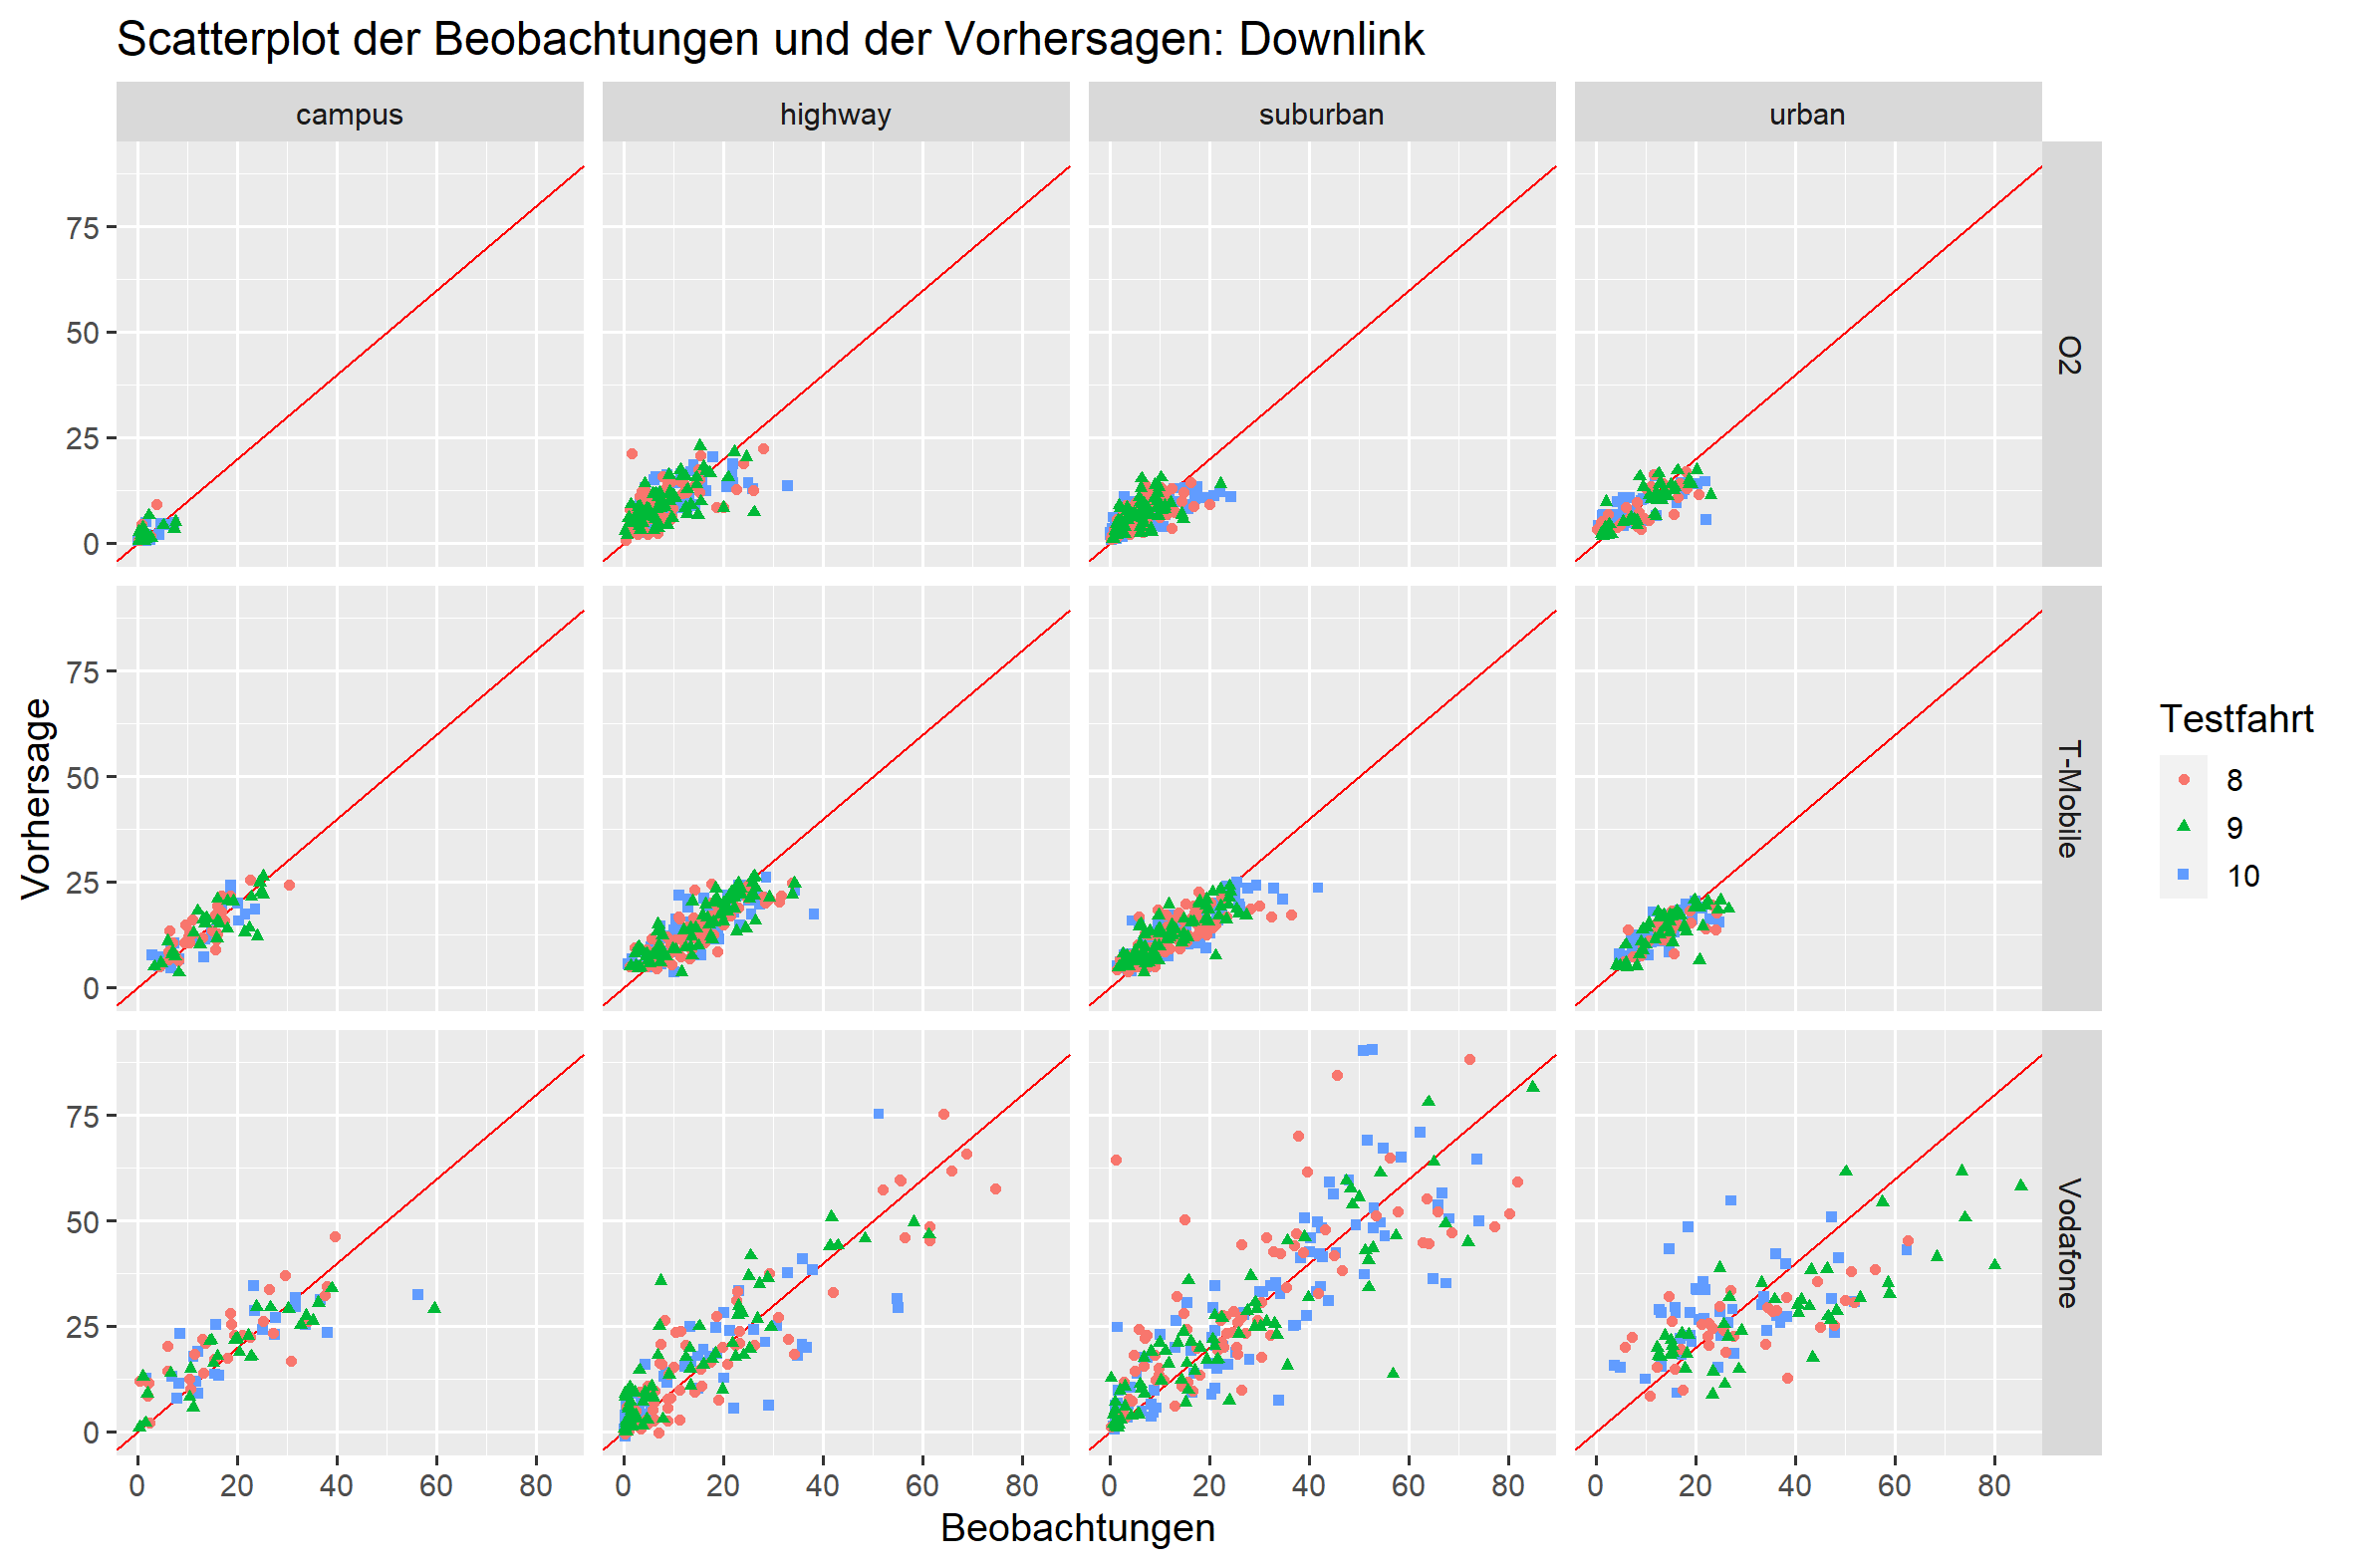
\includegraphics[scale=0.33]{plots/xgboost/downlink/scatter_colored_axes_fixed}
        \caption{XGBoost Out-of-Sample Vorhersagen der Download-Rate}
        \label{xgboost_scatter_colored_downlink}
    \end{figure}
\end{frame}

\subsection{Regression mit ARMA-Fehlern}
\begin{frame}{Regression mit ARMA-Fehlern}
	\underline{Gegeben}: 
	\begin{itemize}
		\item Beobachtungen $(y_1,...,y_T)$ der Zeitreihe $(y_t)_t$
		\item Beobachtungen $(x_1^{(i)},...,x_T^{(i)})$ der Zeitreihen $(x_t^{(i)})_t$ für $i=1,...,k$
	\end{itemize}
	\textbf{Modellgleichung: Regression mit ARMA(p, q)-Fehlern} \cite{forecasting}\\
	\begin{align*}
		y_t &= c + \sum_{j=1}^{k}\beta_j x_t^{(j)} + \eta_t \text{ mit} \\
		\eta_t &= \underbrace{\sum_{k=1}^{p}\phi_p\eta_{t-p}}_{\text{vergangene Fehler: LM}} + \underbrace{\sum_{l=1}^{q}\theta_l\epsilon_{t-q}}_{\text{vergangene Fehler: ARMA}} + \epsilon_{t}
	\end{align*}
\end{frame}

\begin{frame}{Regression mit ARMA-Fehlern}
	Vorarbeit:
	\begin{itemize}
		\item Überprüfung Autokorrelation der Zielvariablen (Acf, pAcf)
		\item Standardisierung Train, Skalierung Test
	\end{itemize}
	Überprüfung der Voraussetzungen:
	\begin{itemize}
		\item Stationarität aller Variablen (Augmented Dickey-Fuller Test)
		\item keine Multikollinearität vorhanden (VIF)
		\item Normalverteilung der Residuen (Scatterplot, Histogramm, QQ-Plot)
	\end{itemize}
\end{frame}

\begin{frame}{Bestimmung des Grids für die AR-Ordnung - Uplink}
		\begin{figure}
			%\centering
			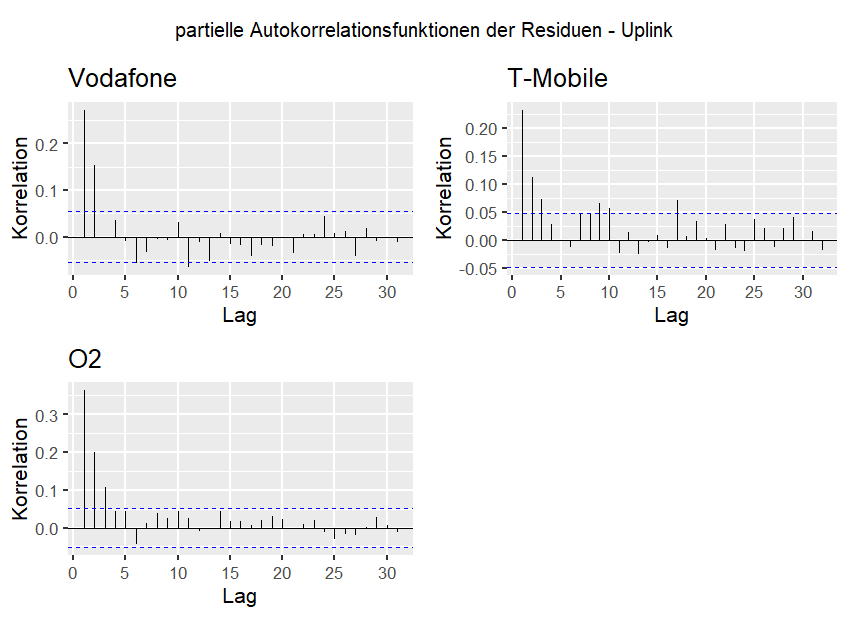
\includegraphics[scale=0.42]{plots/arima/uplink/res_pacf}\\
			\label{res_pacf_ul}
		\end{figure}
\end{frame}

\begin{frame}{Bestimmung des Grids für die MA-Ordnung - Uplink}
		\begin{figure}
			%\centering
			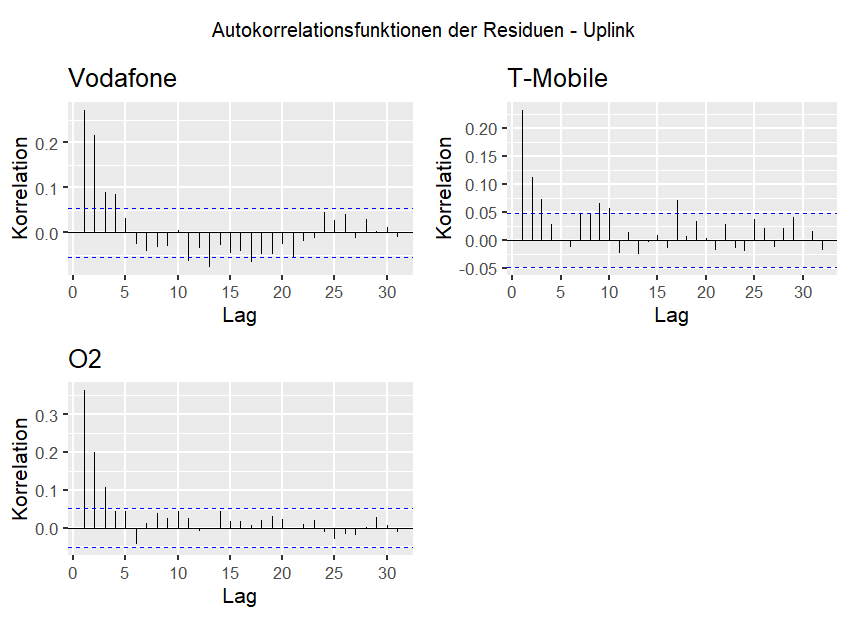
\includegraphics[scale=0.42]{plots/arima/uplink/res_acf}\\
			\label{res_acf_ul}
		\end{figure}
\end{frame}

\begin{frame}{Regression mit ARMA-Fehlern: Ergebnisse (Uplink)}
	\begin{figure}
		\centering
		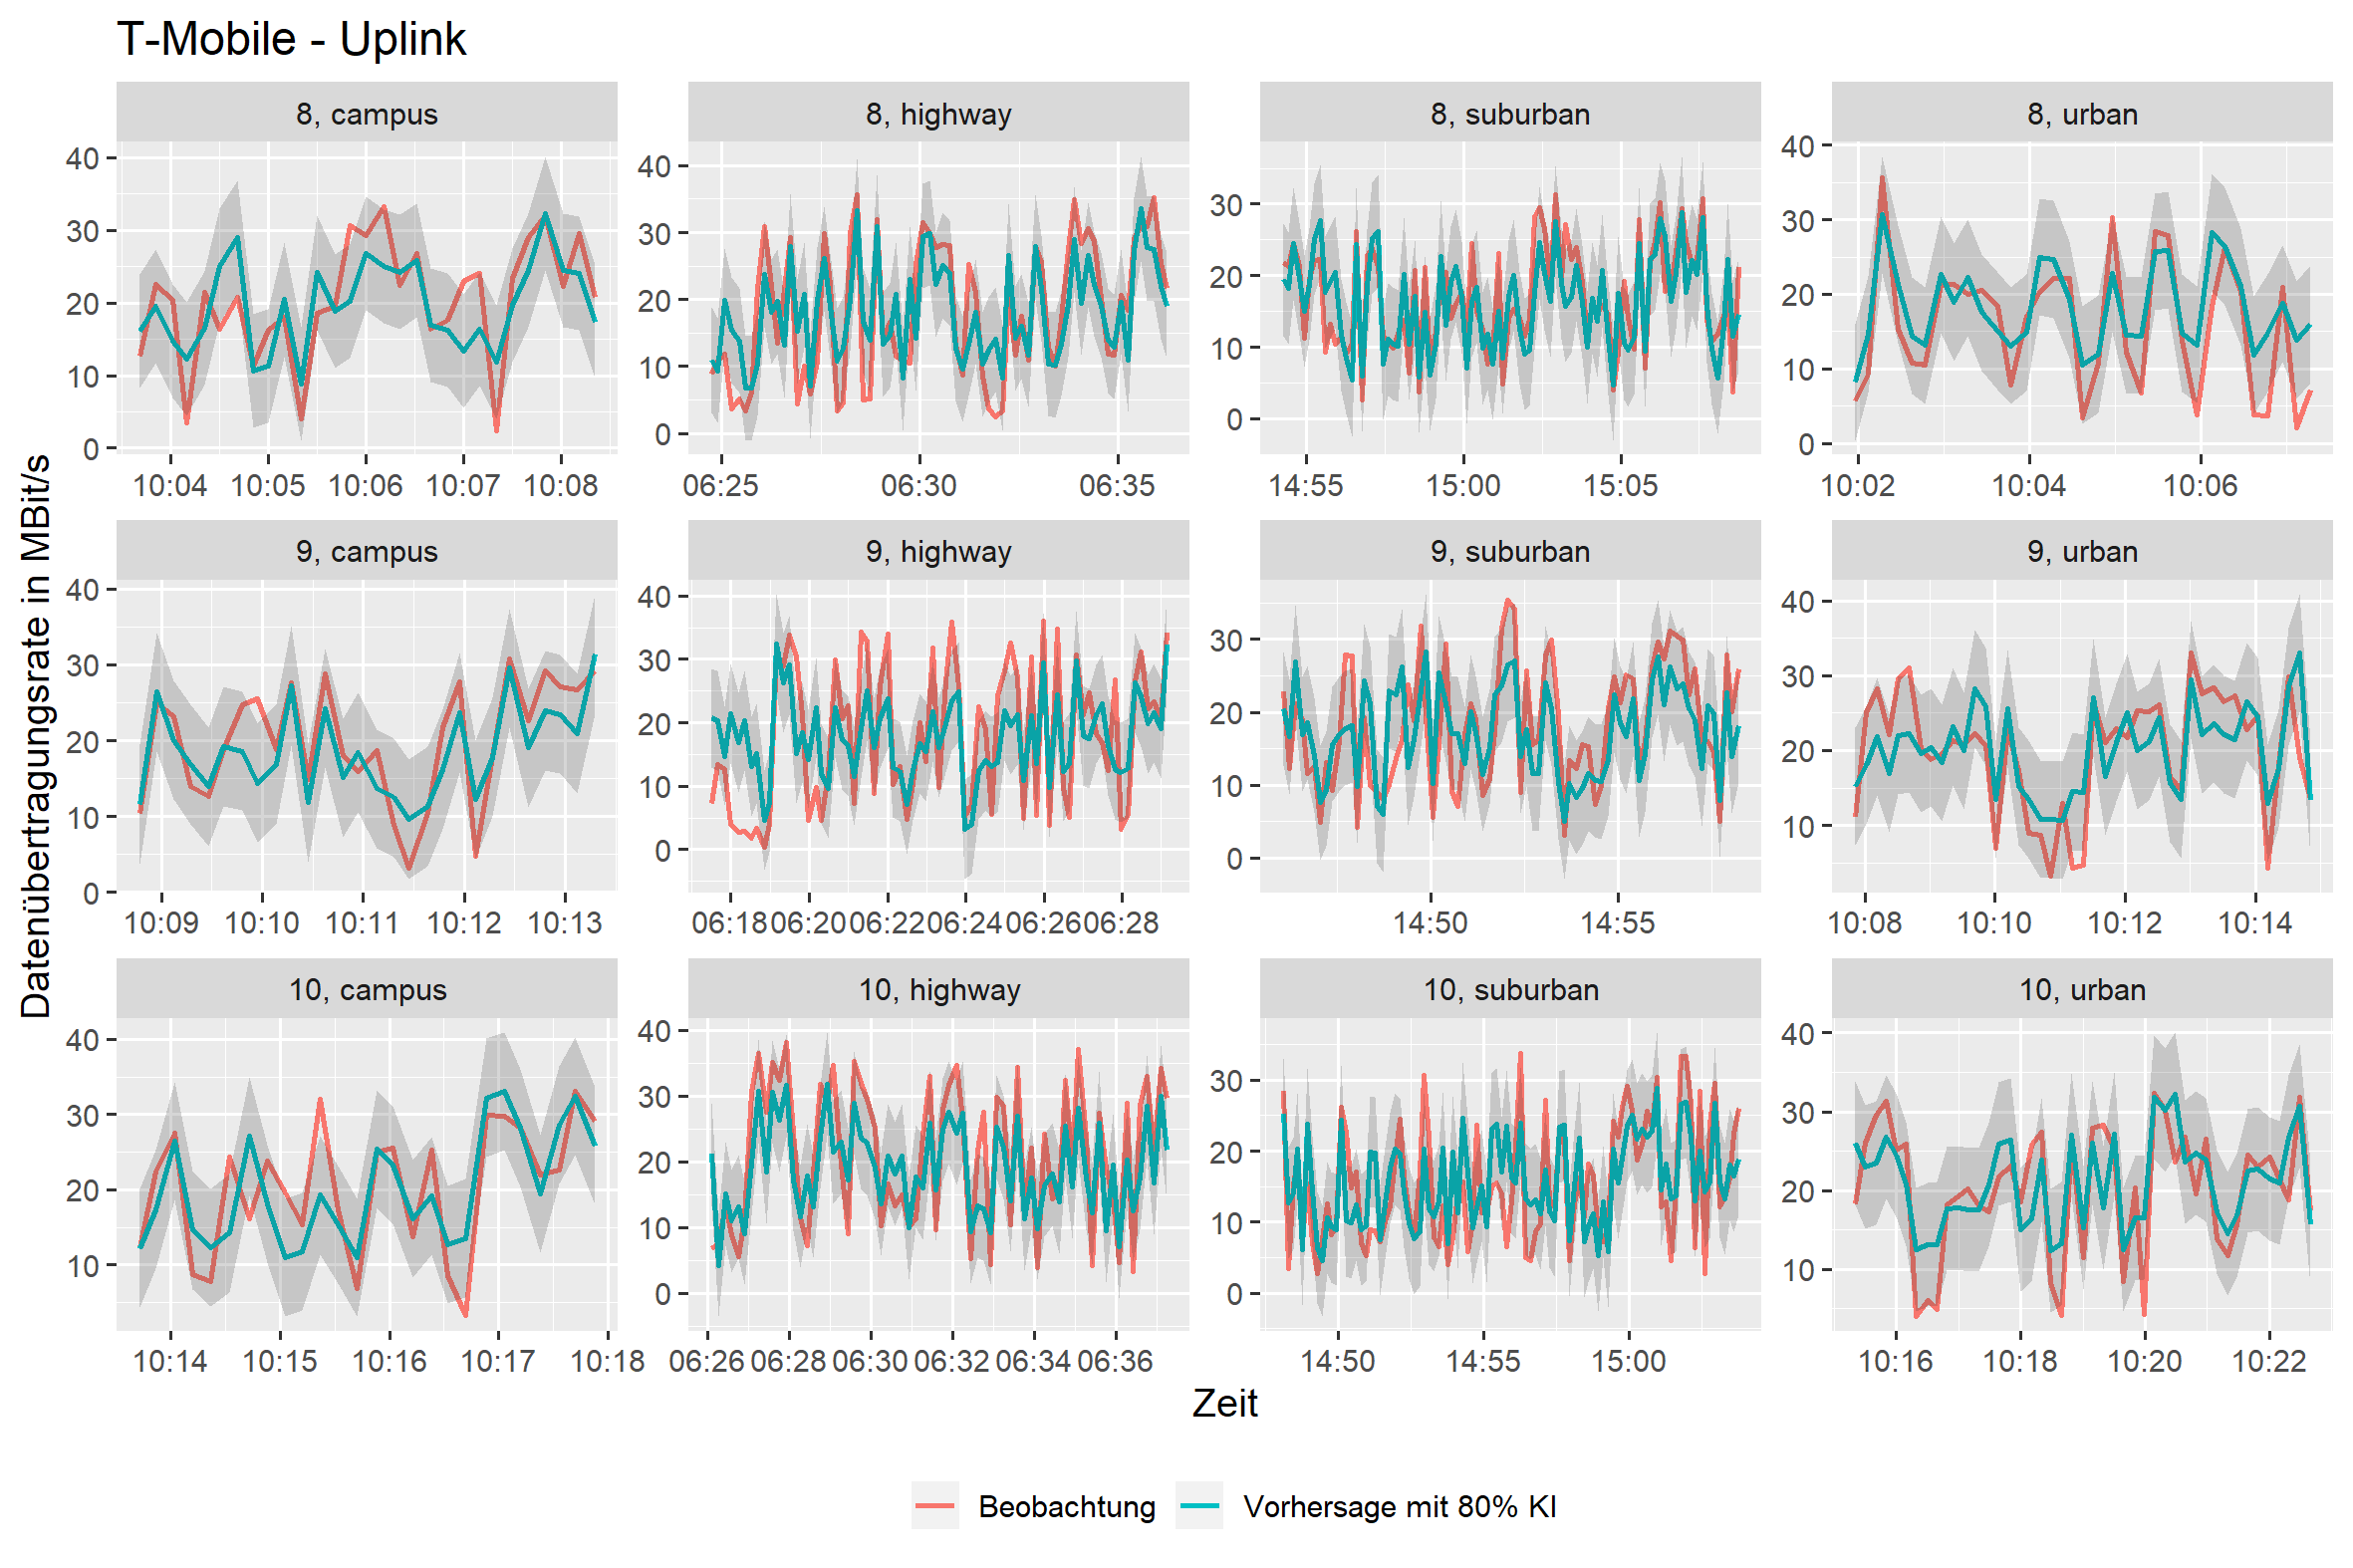
\includegraphics[scale=0.38]{plots/arima/uplink/tmobile_predictions}\\
		\caption{Vorhersage der Datenübertragungsrate des Providers T-Mobile in Richtung Uplink.}
		\label{tmobile_predictions_ul}
	\end{figure}
\end{frame}

\begin{frame}{Regression mit ARMA-Fehlern: Ergebnisse (Uplink)}
	\begin{figure}
		\centering
		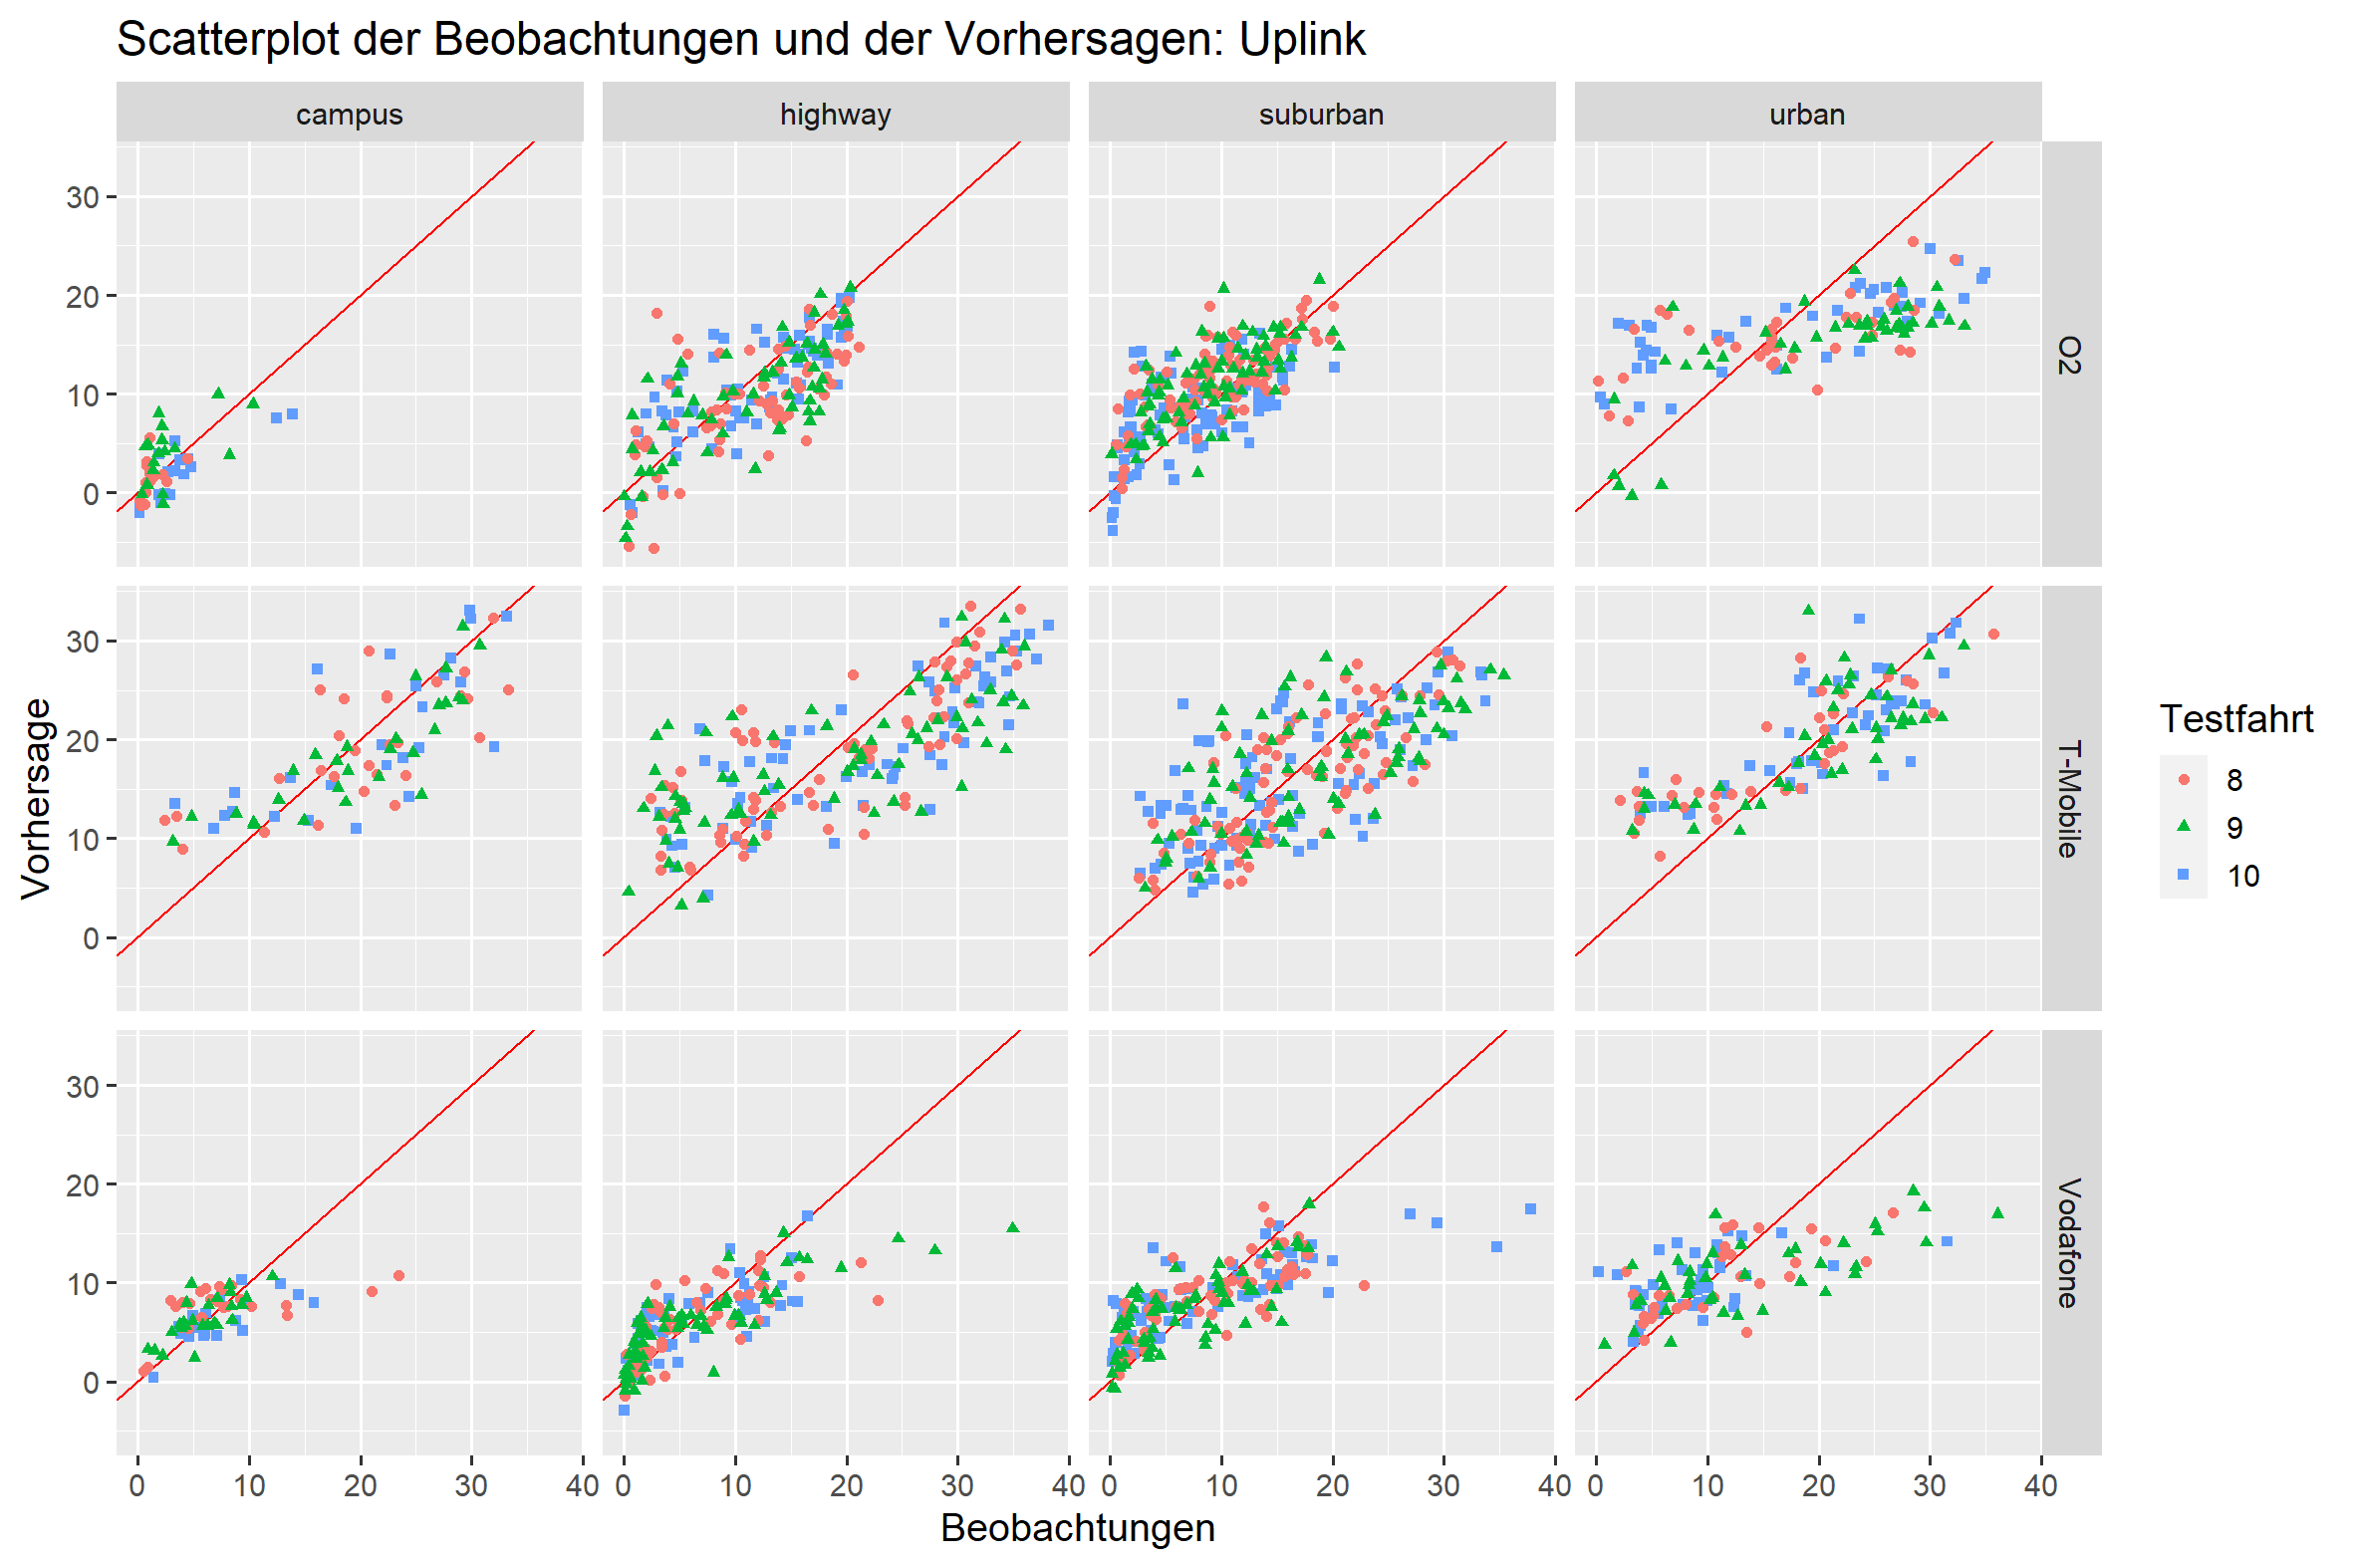
\includegraphics[scale=0.38]{plots/arima/uplink/scatter_colored_axes_fixed}\\
		\caption{Scatterplots der Vorhersagen und Beobachtungen für alle Szenarien und alle Provider in Richtung Uplink.}
		\label{arima_scatter_ul}
	\end{figure}
\end{frame}

\begin{frame}{Regression mit ARMA-Fehlern: Ergebnisse (Downlink)}
	\begin{figure}
		\centering
		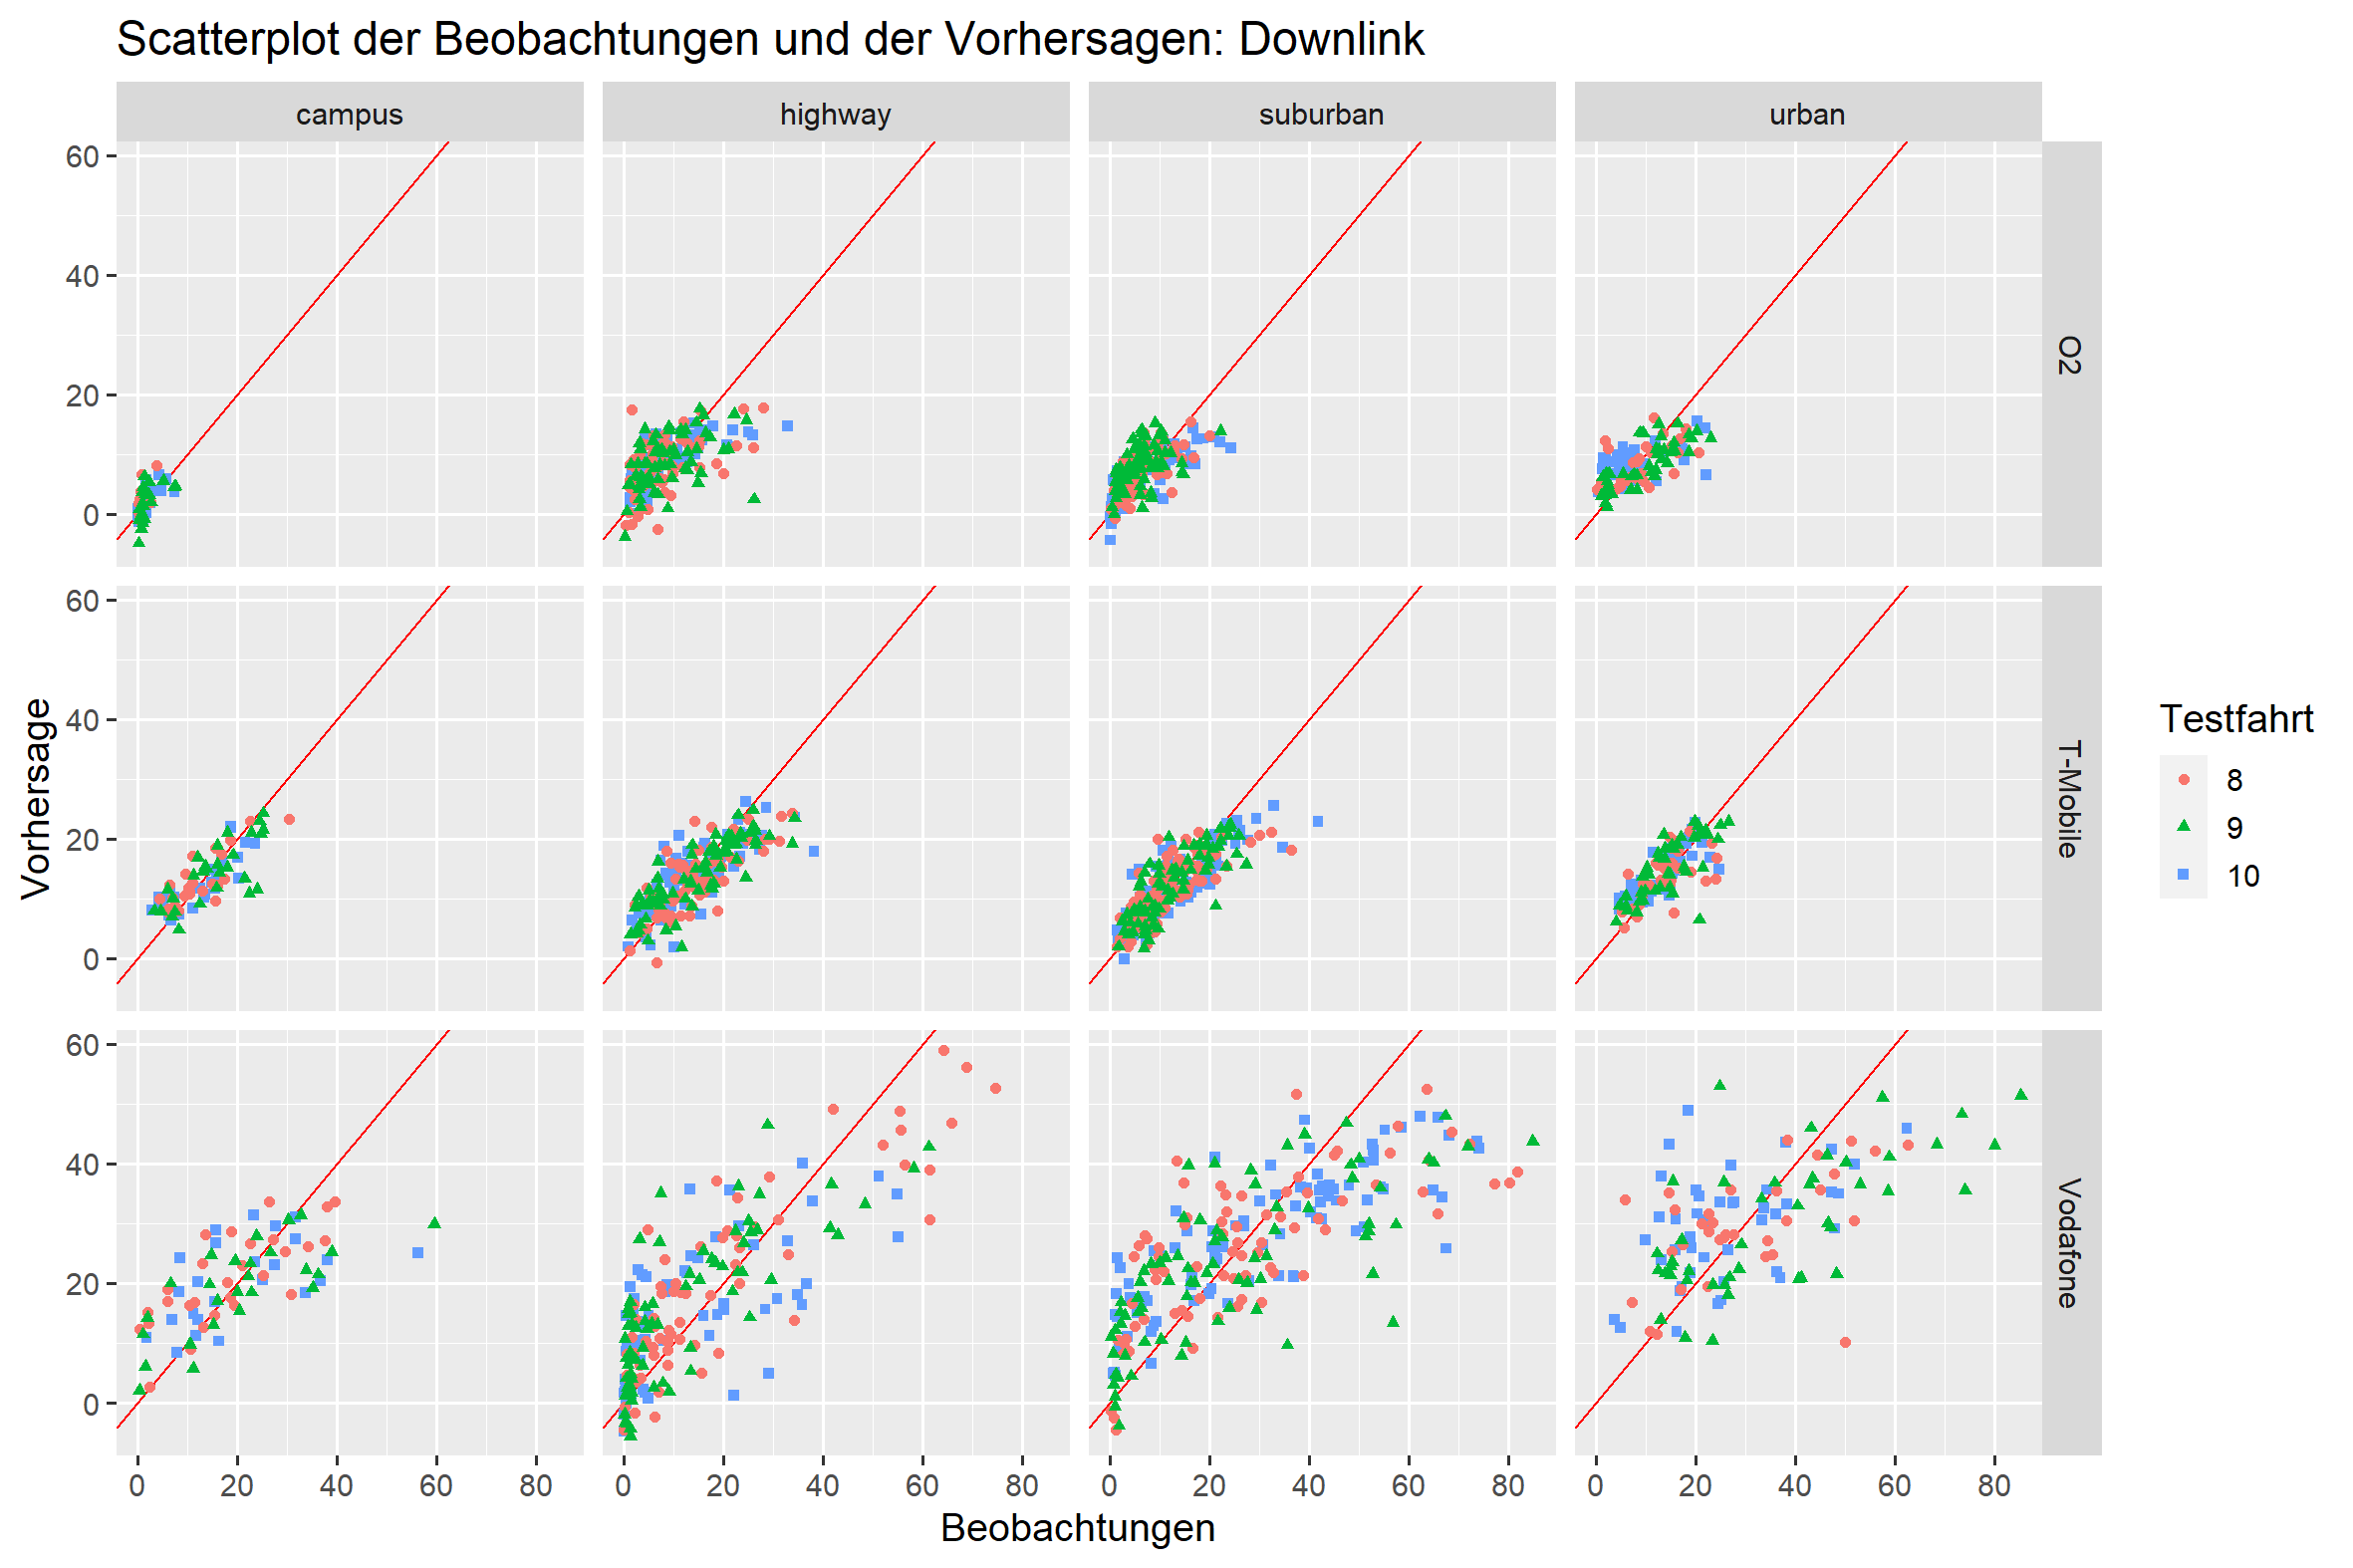
\includegraphics[scale=0.38]{plots/arima/downlink/scatter_colored_axes_fixed}\\
		\caption{Scatterplots der Vorhersagen und Beobachtungen für alle Szenarien und alle Provider in Richtung Downlink.}
		\label{arima_uplink_scatter}
	\end{figure}
\end{frame}




	




\subsection{Modellvergleich}


\begin{frame}{Modellvergleich Uplink - Kennzahlen}
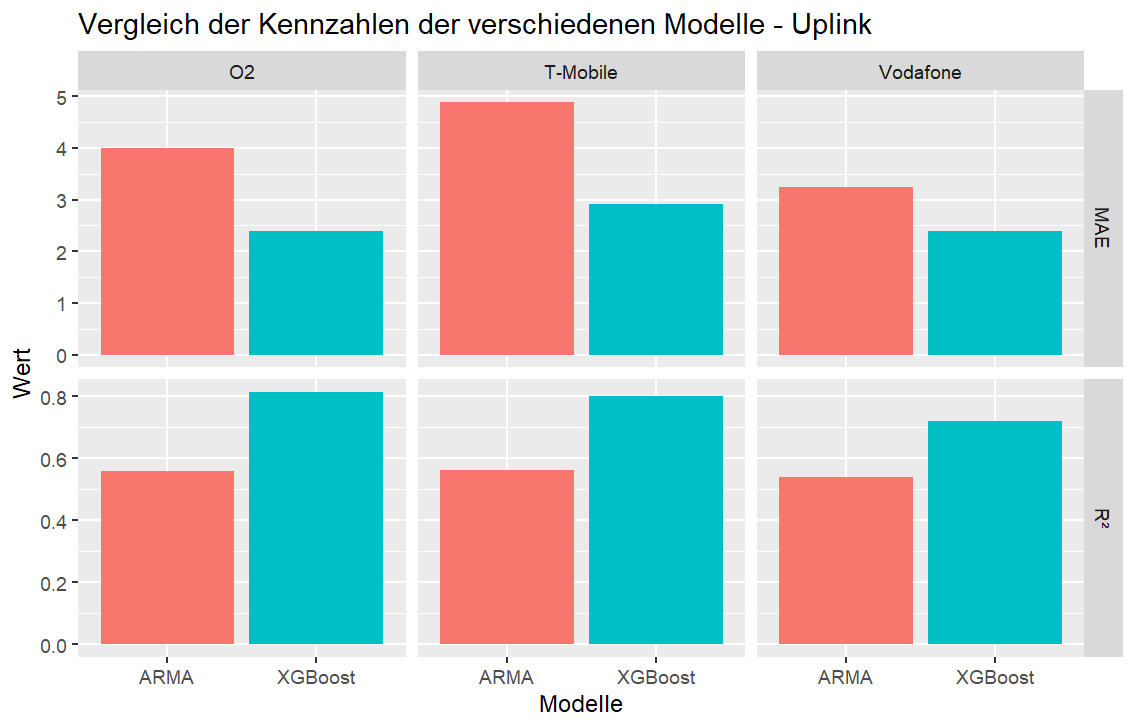
\includegraphics[width = 11cm]{plots/kennzahlen_vergleich_uplink}
\end{frame}

\begin{frame}{Modellvergleich Downlink - Kennzahlen}
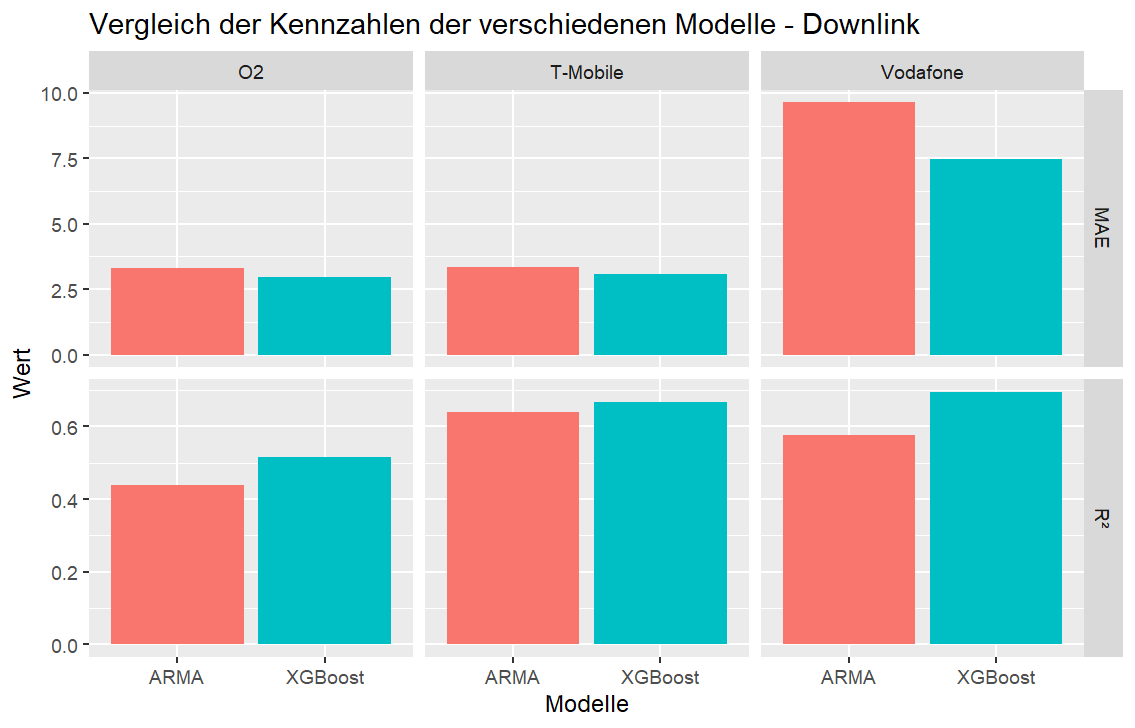
\includegraphics[width = 11cm]{plots/kennzahlen_vergleich_downlink}
\end{frame}


\begin{frame}{Modellvergleich Uplink - Feature Importance}
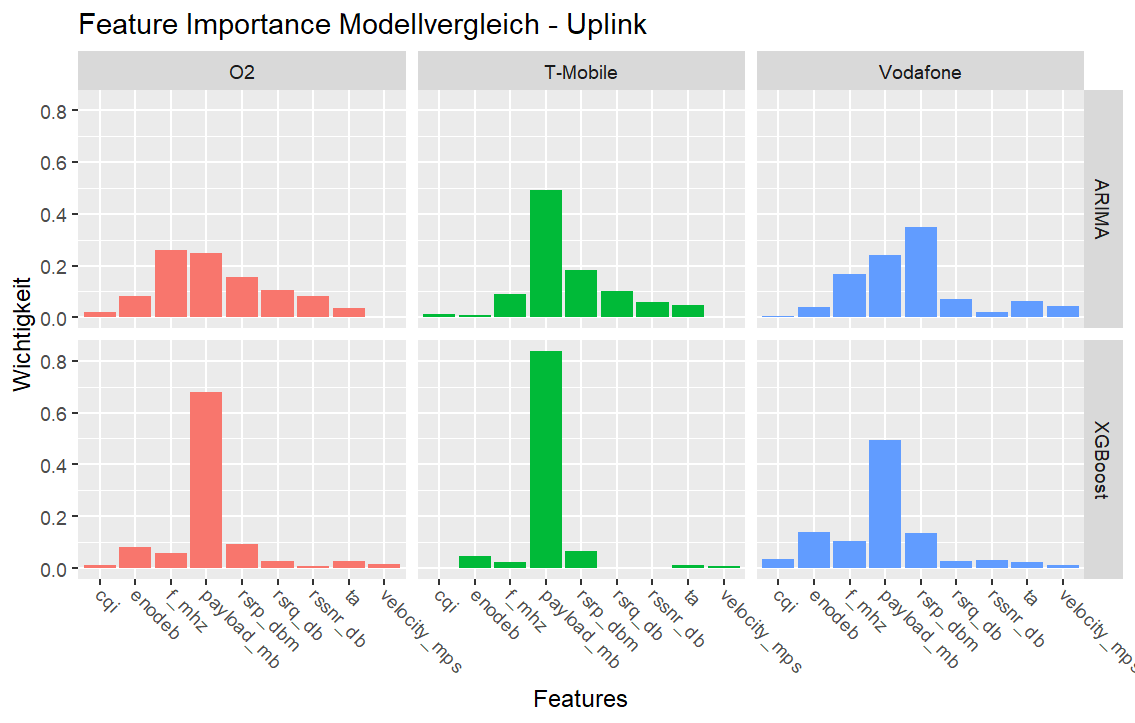
\includegraphics[width = 11cm]{plots/feature_importance_modellvergleich_uplink}
\end{frame}


\begin{frame}{Methodenvergleich XGBoost - Uplink}
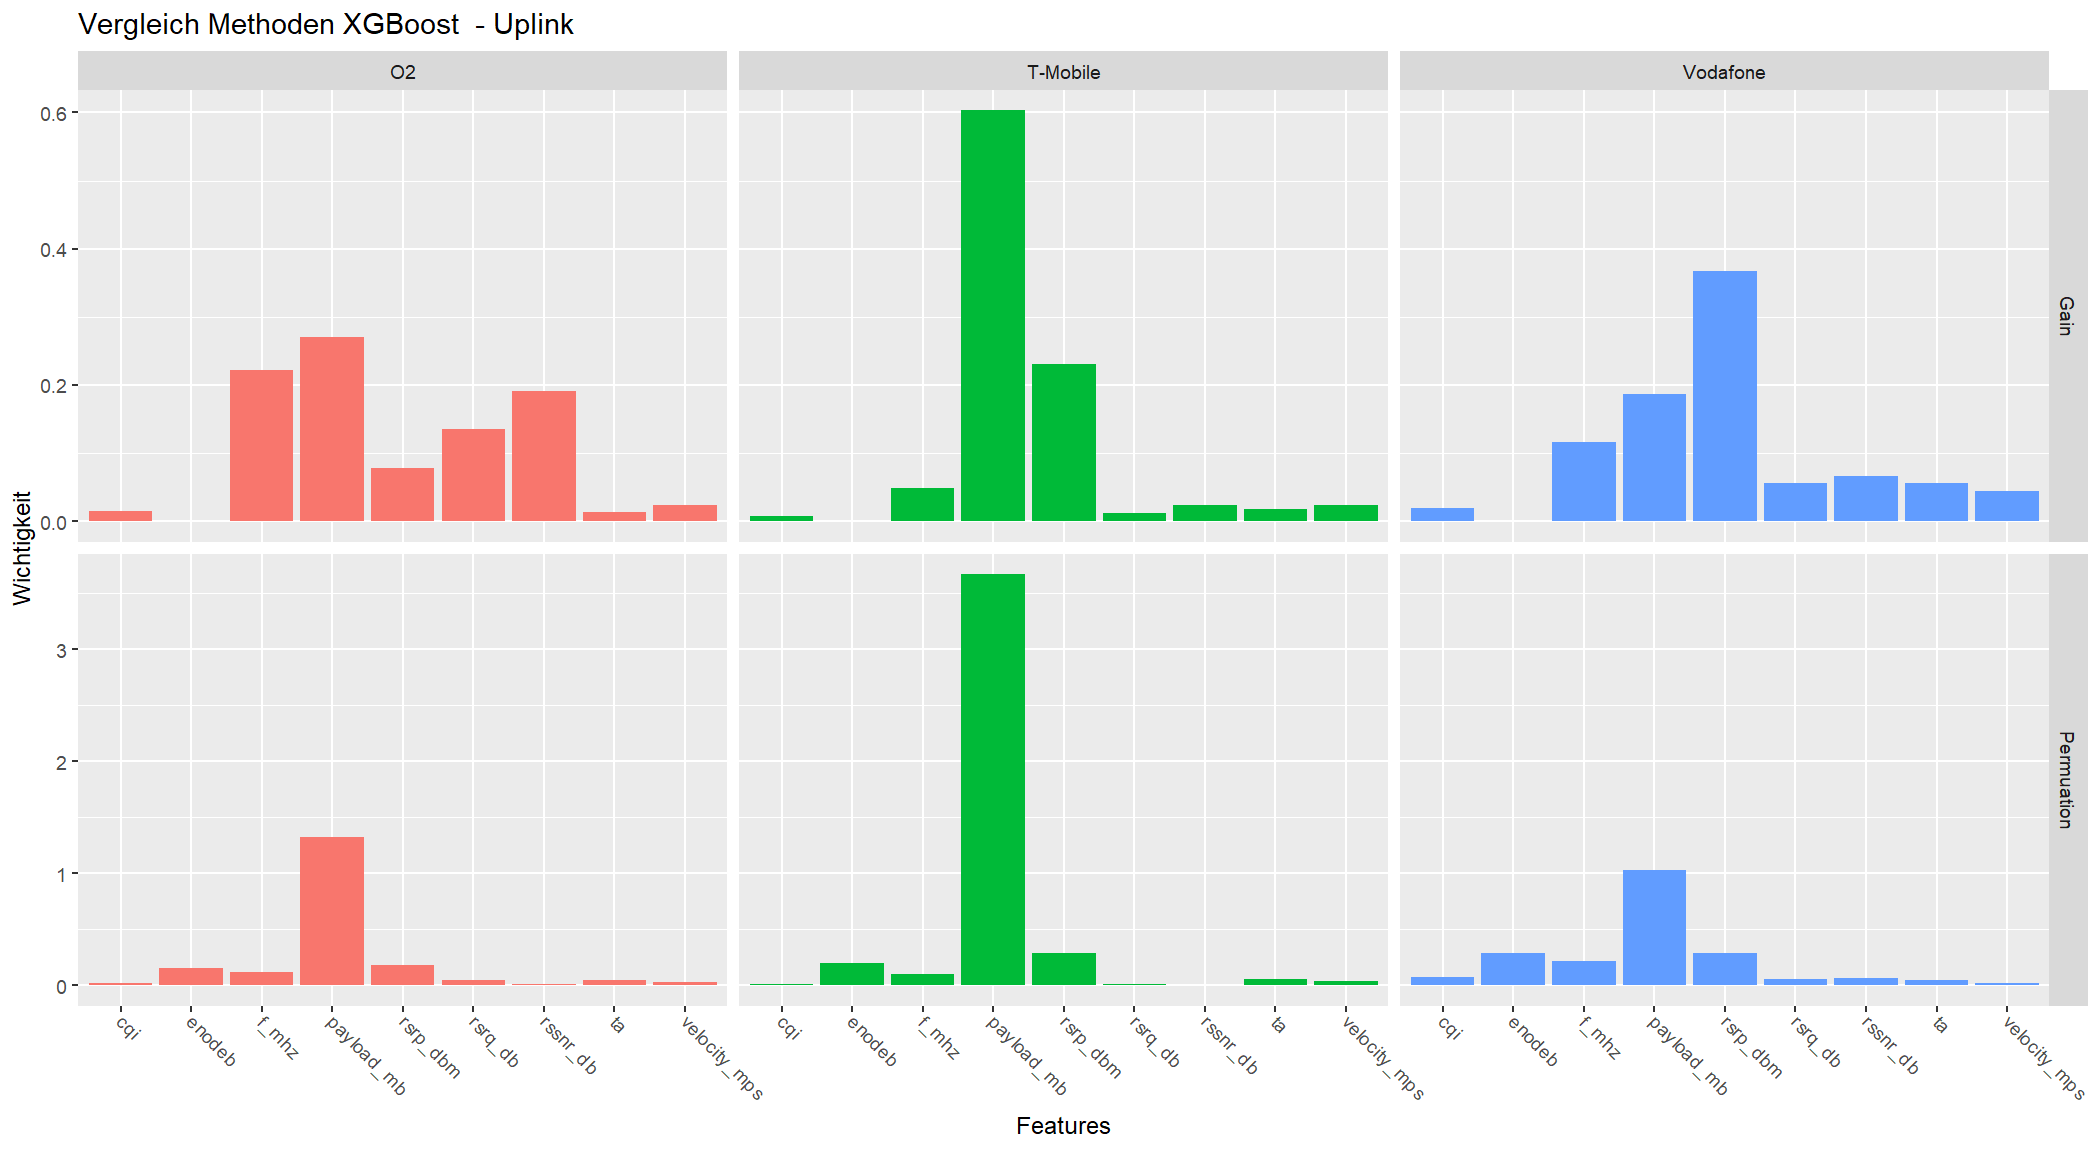
\includegraphics[width = 11cm]{plots/gainvspermutation_uplink}
\end{frame}

\begin{frame}{Modellvergleich Downlink - Feature Importance}
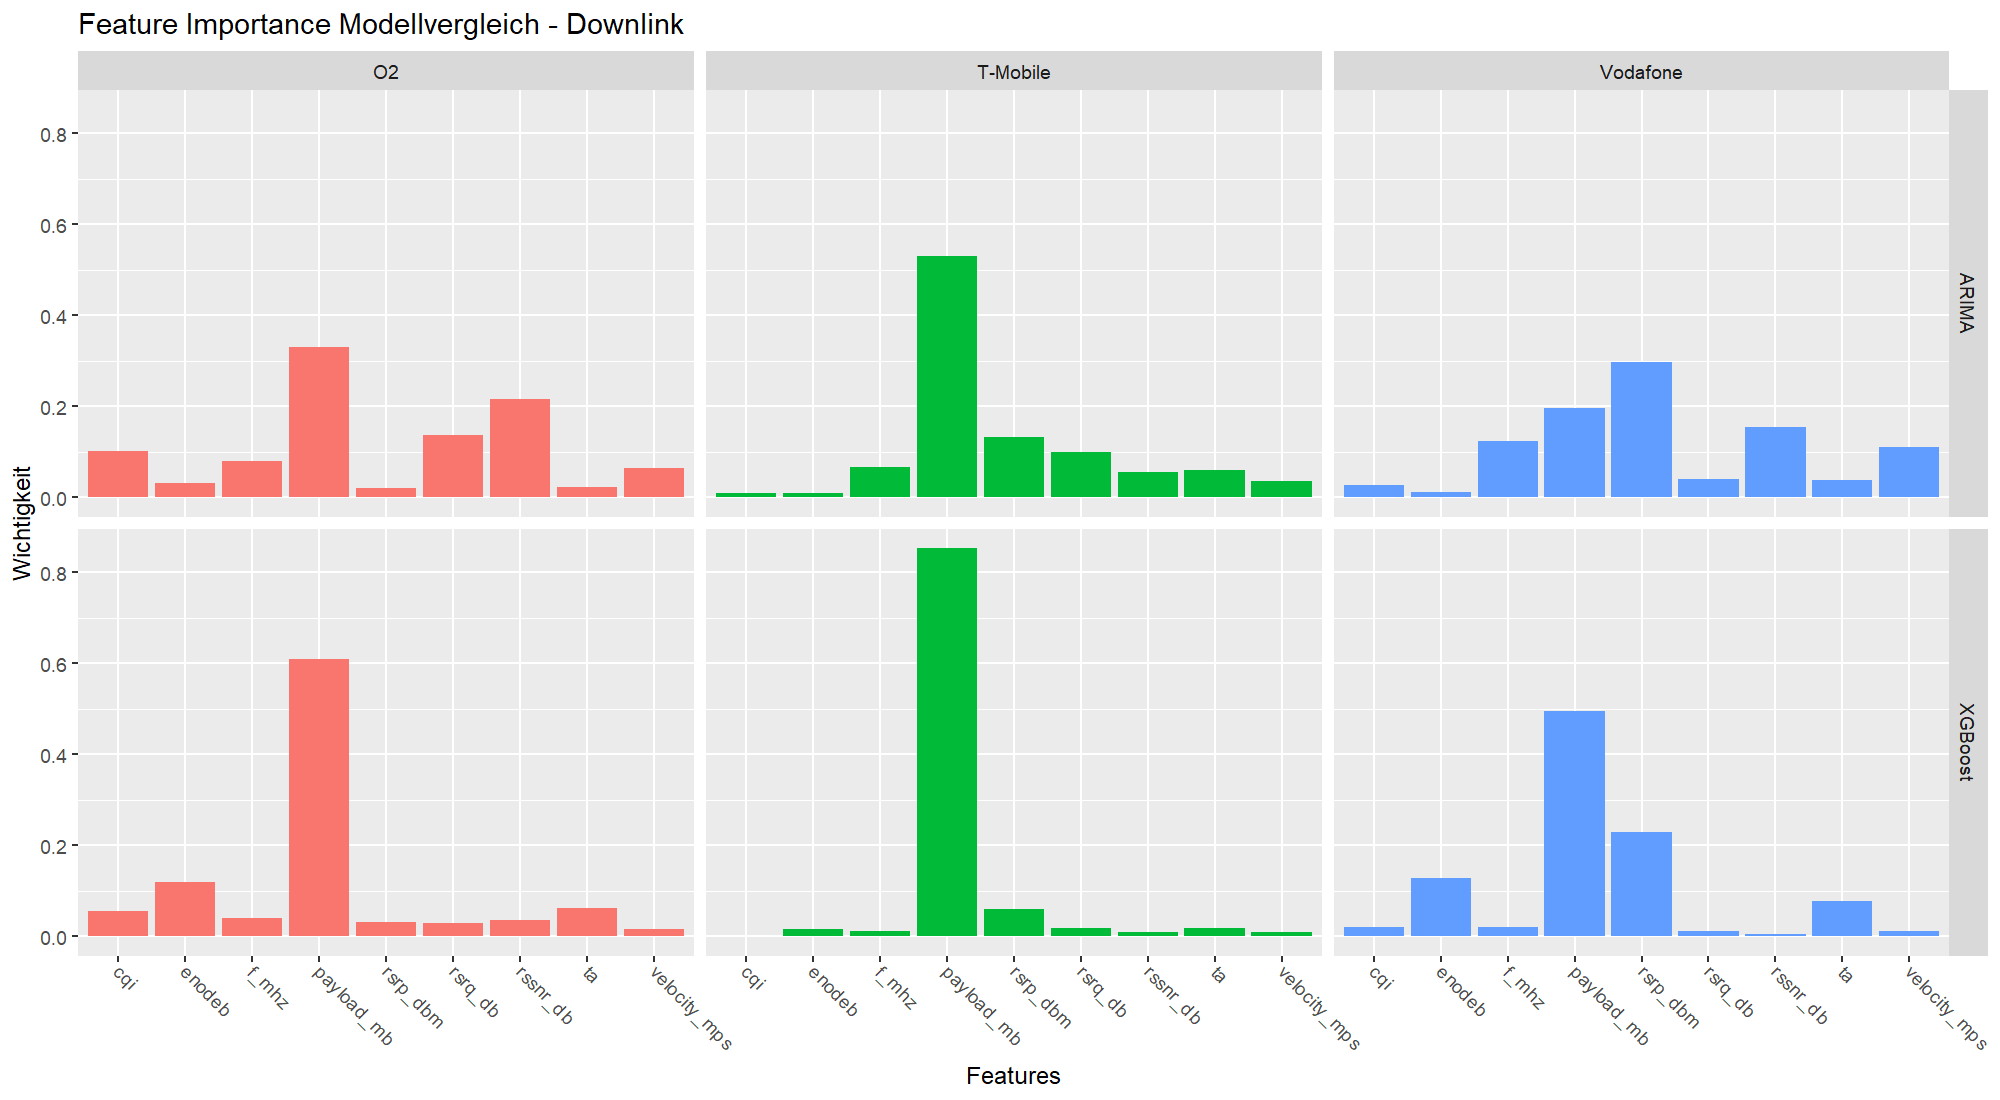
\includegraphics[width = 11cm]{plots/feature_importance_modellvergleich_downlink}
\end{frame}


\begin{frame}{Methodenvergleich XGBoost - Downlink}
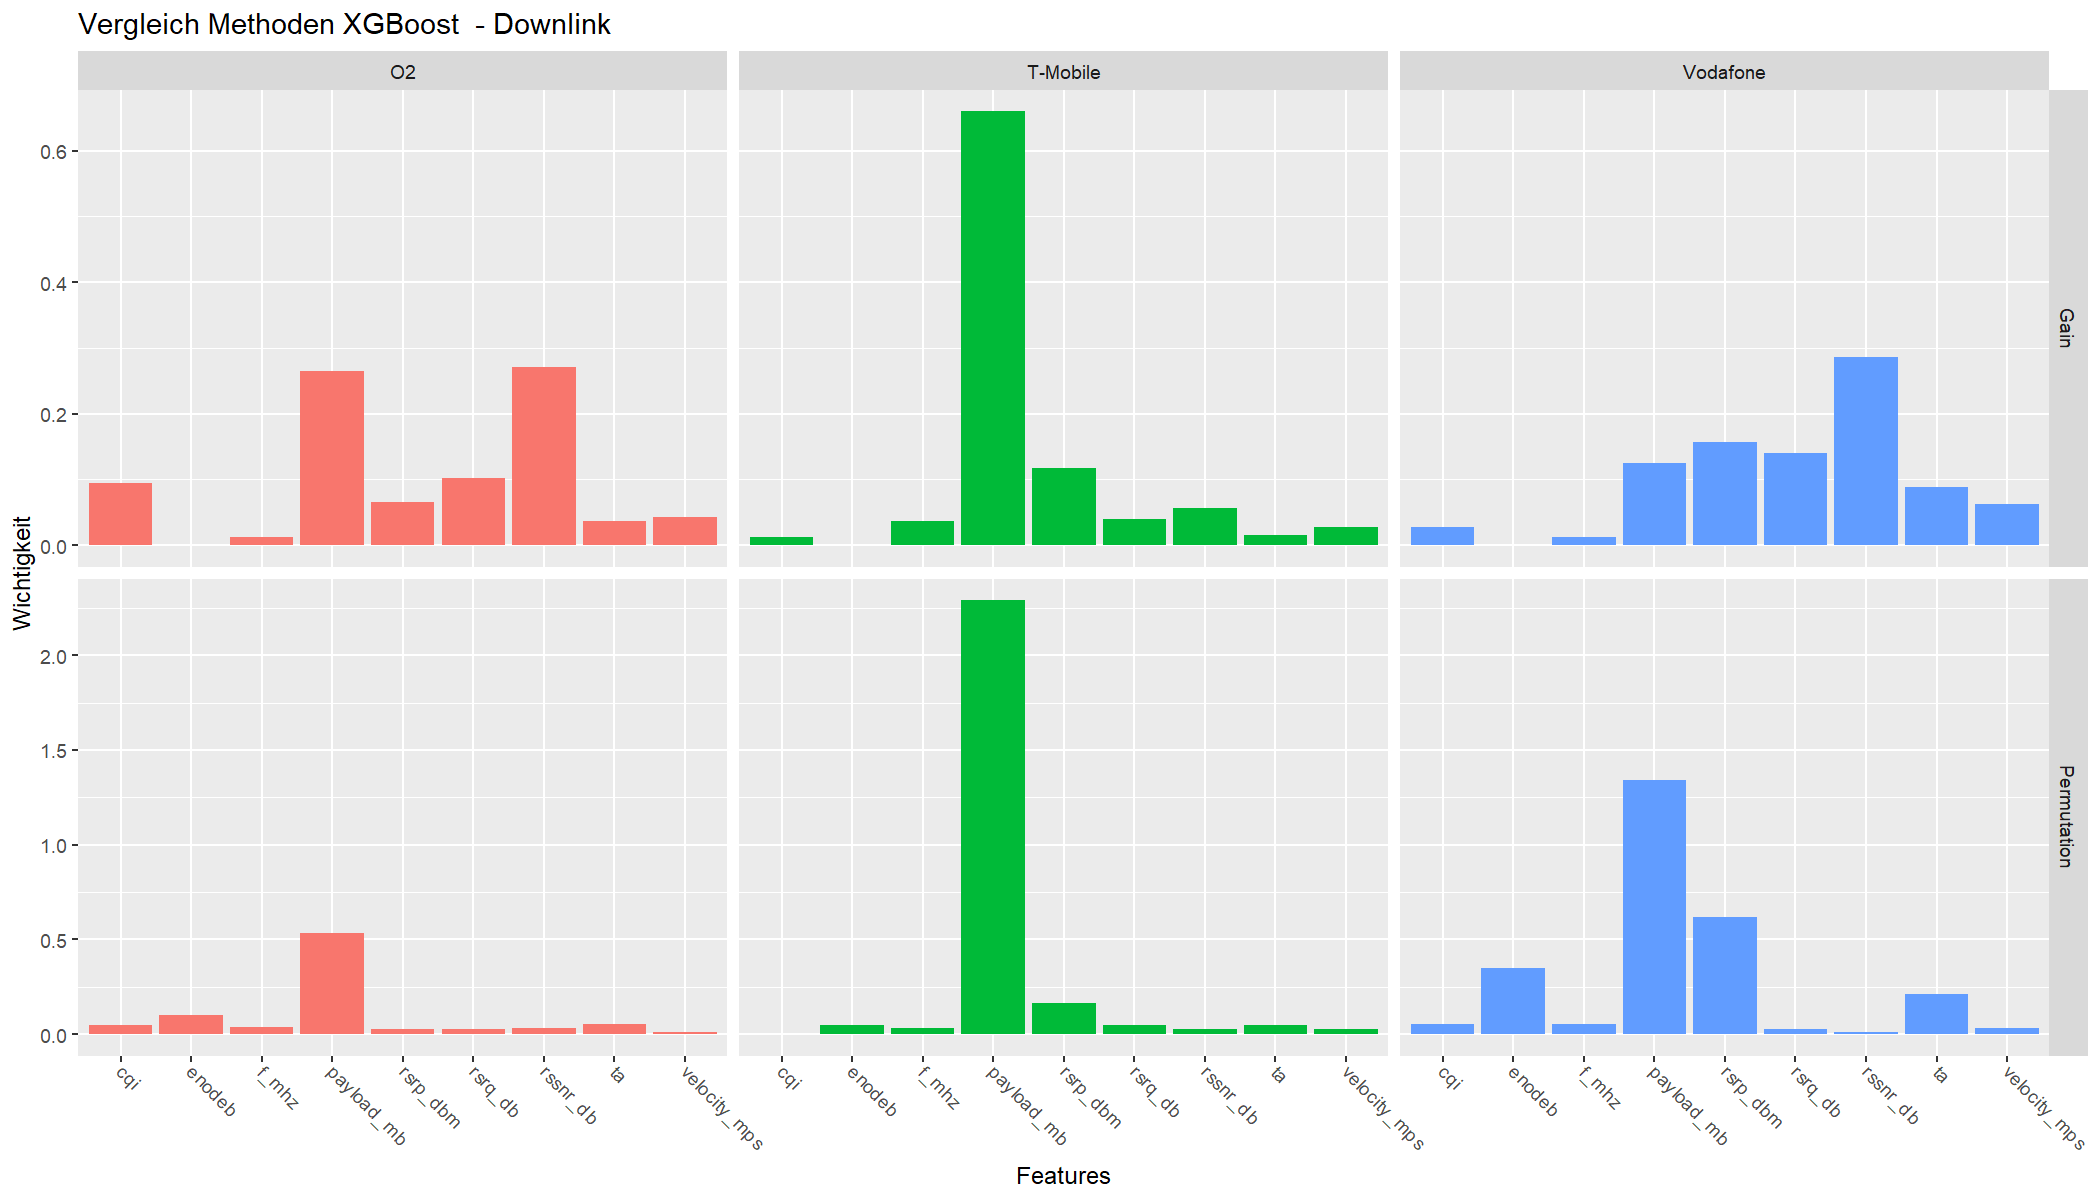
\includegraphics[width = 11cm]{plots/gainvspermutation_downlink}
\end{frame}








\section{TaskII}
\begin{frame}{frame}
hallo 
\end{frame}

\subsection{Feature Importance}


\begin{frame}{Feature Importance}
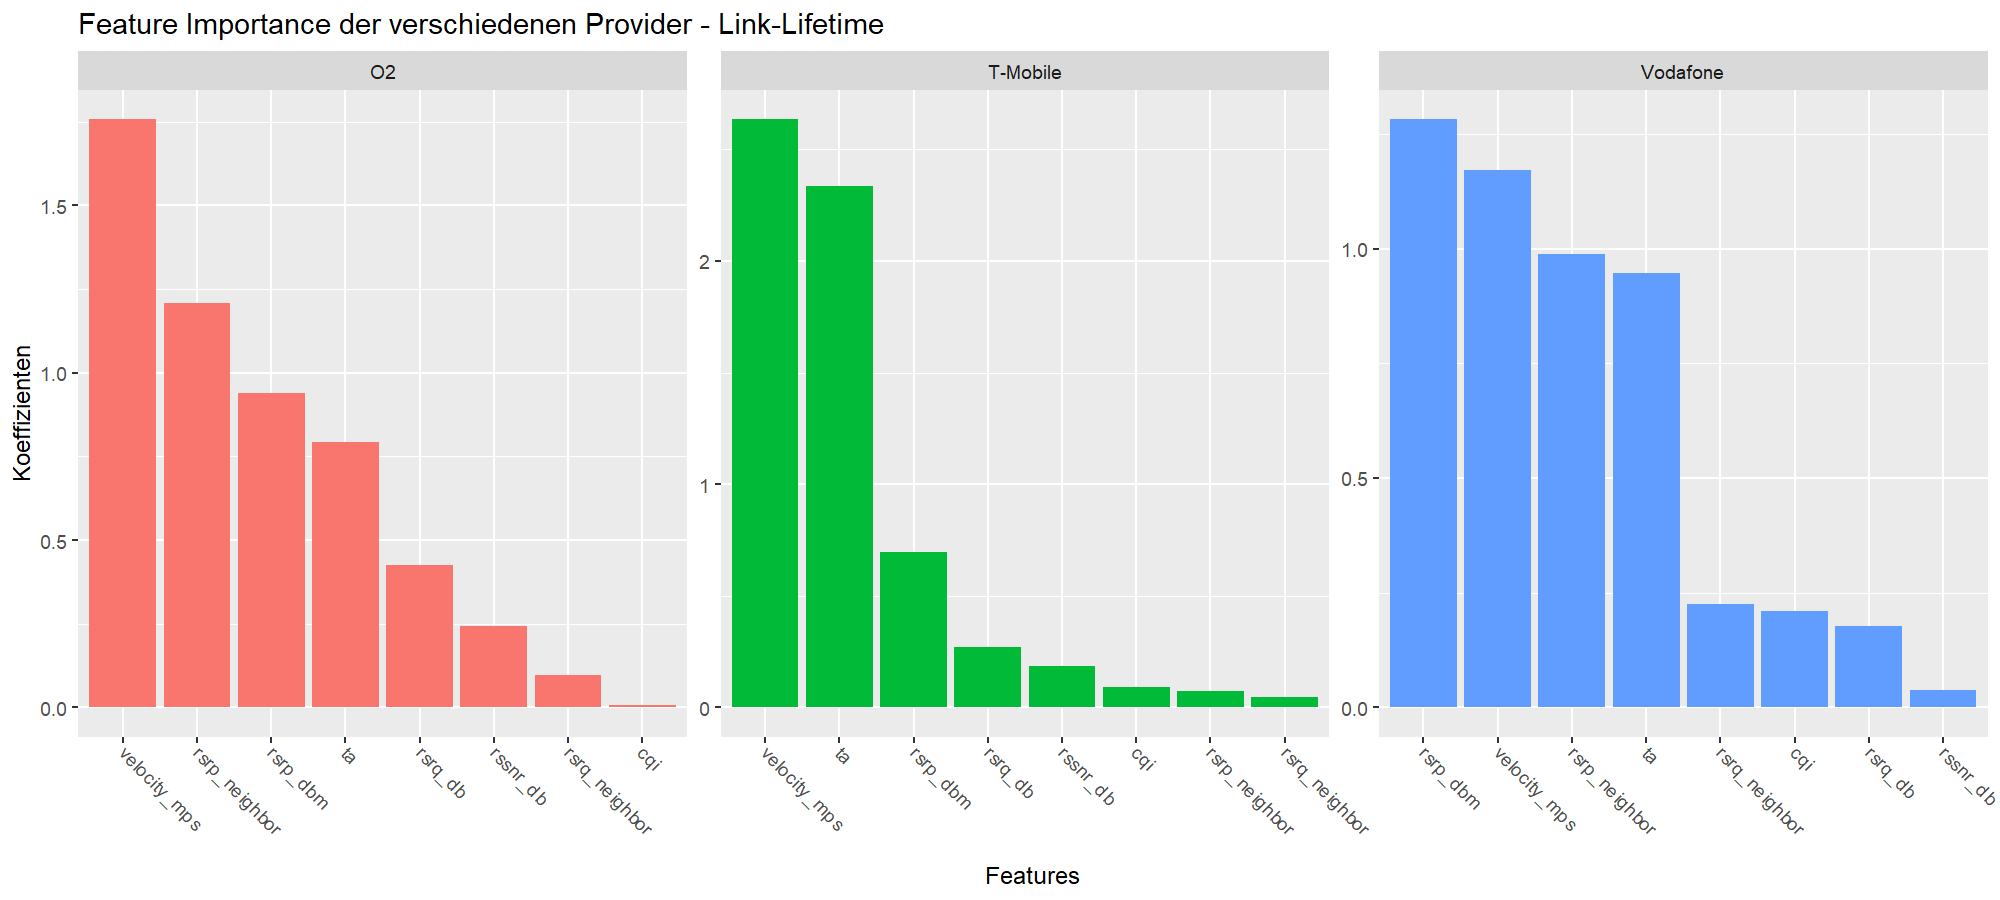
\includegraphics[width = 11cm]{plots/link_lifetime/feature_importance}
\end{frame}



%\begin{frame}[standout]
%  Irgendwas zum Schluss
%\end{frame}

\appendix

\begin{frame}[allowframebreaks]{Literatur}

  \nocite{XGBoost}

  \bibliography{literatur}
  \bibliographystyle{abbrv}

\end{frame}

\begin{frame}{Regression mit ARMA-Fehlern}
	\textbf{h-Schritt Punktvorhersage}\\
	\begin{itemize}
		\item Ersetze Beobachtungen zu zukünftigen Zeitpunkten mit deren Vorhersagen
		\item Ersetze Fehler an vergangenen Zeitpunkten durch das entsprechende Residuum
		\item Ersetze Fehler an zukünftigen Zeitpunkten durch 0
	\end{itemize}
	\underline{Beispiel}: $h=2, k=1, p=2, q=2$
	\begin{alignat*}{2}
		y_t &= c + \beta_1 x_{t} + \epsilon_t \text{ mit }&&\epsilon_{t} = \phi_1\epsilon_{t-1} + \phi_2\epsilon_{t-2} + \theta_1e_{t-1} + \theta_2e_{t-2} + e_t \\		
		\widehat{y_{t+1}} &= c + \beta_1 x_{t} + \widehat{\epsilon_{t+1}} \text{ mit }&& \widehat{\epsilon_{t+1}} = \phi_1\epsilon_{t} + \phi_2\epsilon_{t-1} + \theta_1e_{t} + \theta_2e_{t-1} + \underbrace{\widehat{e_{t+1}}}_{=0}\\
		\widehat{y_{t+2}} &= c + \beta_1 x_{t} + \widehat{\epsilon_{t+2}}\text{ mit }&&\widehat{\epsilon_{t+2}} = \phi_1\widehat{\epsilon_{t+1}} + \phi_2\epsilon_t + \theta \underbrace{\widehat{e_{t+1}}}_{=0} + \theta e_t + \underbrace{\widehat{e_{t+2}}}_{=0}
	\end{alignat*}
\end{frame}

\begin{frame}{Gradient Boosted Trees}
    \begin{itemize}
        \item Kann man aus vielen \glqq schwachen \grqq{} Lernern einen starken Lerner konstruieren?
            \begin{itemize}
                \item[$\Rightarrow$] Ja, Boosting ist eines der m\"achtigsten Konzepte des Machine Learning \cite{elements}
            \end{itemize}
        \item Kombination von einfachen CART B\"aumen zu einem starken Ensemble
            \begin{itemize}
                \item[$\Rightarrow$] \"Ahnlich zu Random Forest
            \end{itemize}
        \item Der Unterschied zum Random Forest liegt im Training!
    \end{itemize}
\end{frame}

\begin{frame}{Training von Gradient Boosted Trees}
    \begin{itemize}
        \item B\"aume werden nacheinander zum Ensemble hinzugef\"ugt
        \item Jeder neue Baum versucht, die Schw\"achen seiner Vorg\"anger "auszub\"ugeln"
            \begin{itemize}
                \item[$\Rightarrow$] \textit{Additives Training}
            \end{itemize}
        \item Je mehr B\"aume aufgenommen werden, desto geringer wird der Training-Error (das Modell wird aber komplexer)
            \begin{itemize}
                \item[$\Rightarrow$] Kontrolle des \textit{Bias-Variance Tradeoffs}
                \item[$\Rightarrow$] Zus\"atzlich gibt es Regularisierungs-Parameter
            \end{itemize}
    \end{itemize}
\end{frame}

\begin{frame}{Implementierung: XGBoost}
    \begin{itemize}
        \item Liefert state-of-the-art Performance in einer Vielzahl von ML-Problemen
        \item In 2015 haben 19/25 Gewinner von Kaggle-Competitions XGBoost eingesetzt
        \item Kann problemlos auf mehrere Milliarden Training Samples skaliert werden 
        \item L\"asst sich aber auch hervorragend auf ressourcenbegrenzten Systemen einsetzen \cite{XGBoost}
    \end{itemize}
\end{frame}

\end{document}
